\chapter{Results}


\section{Shear Wave Decay}
The Shear Wave Decay is a common concept in computational physics to measure the kinematic viscosity of a fluid.
It is set up by creating an initial sinusoidal velocity profile and measuring the decay rate.
The field is set up without any borders, which results in e.g.\ particles moving out of the right to appear back on the left side.
The default parameters for the Shear Wave Decay experiments are shown in \cref{tab:swd-parameters} and used if not stated otherwise.

\begin{table}[ht]
    \centering % used for centering table
    \begin{tabular}{c c}
% centered columns (4 columns)
        \hline\hline %inserts double horizontal lines
        Parameter  & Value \\ [0.5ex] % inserts table heading
        \hline % inserts single horizontal line
        $L_x$      & 100   \\
        $L_y$      & 100   \\
        $\omega$   & 1.0   \\
        $\epsilon$ & 0.01  \\
        $t_{\max}$ & 1000  \\ [1ex] % [1ex] adds vertical space
        \hline %inserts single line
    \end{tabular}
    \caption{Parameters for the Shear Wave Decay} % title of Table
    \label{tab:swd-parameters}
\end{table}

\subsection{Sinusodial Density}
The initial condition is a given by the following equation where $L_x$ resembles the size in x-direction

\begin{equation*}
    \begin{aligned}
        \mathbf{u}(\mathbf{r},0) &= 0 \\
        \rho(\mathbf{r},0) &= \rho_0 + \epsilon \sin \left( \frac{2 \pi x}{L_x} \right) \cdot
    \end{aligned}
\end{equation*}

Because of the initialization the fluid is shaped like a sinusoid wave without any velocity.
It is expected that this wave collapses in itself.
This is due to the fact that the system tries to reach a state of equilibrium where the mass at each position is the same.
Therefore, a flow is created from the higher density area to the lower density area.
This flow continues until the mass at the previous lower density area is so dense, that no further flow is created. %TODO better explaining why it overflows!
It now reached a state similar to the beginning however the dense and low-dense areas swapped which is why the flow will have opposite directions in the next iteration.
This process can be seen in \cref{fig:swd-stream-velocity}. % TODO fix formatting (text-image-text-image)

\begin{figure}[h!]
    \begin{minipage}{0.33\textwidth}
        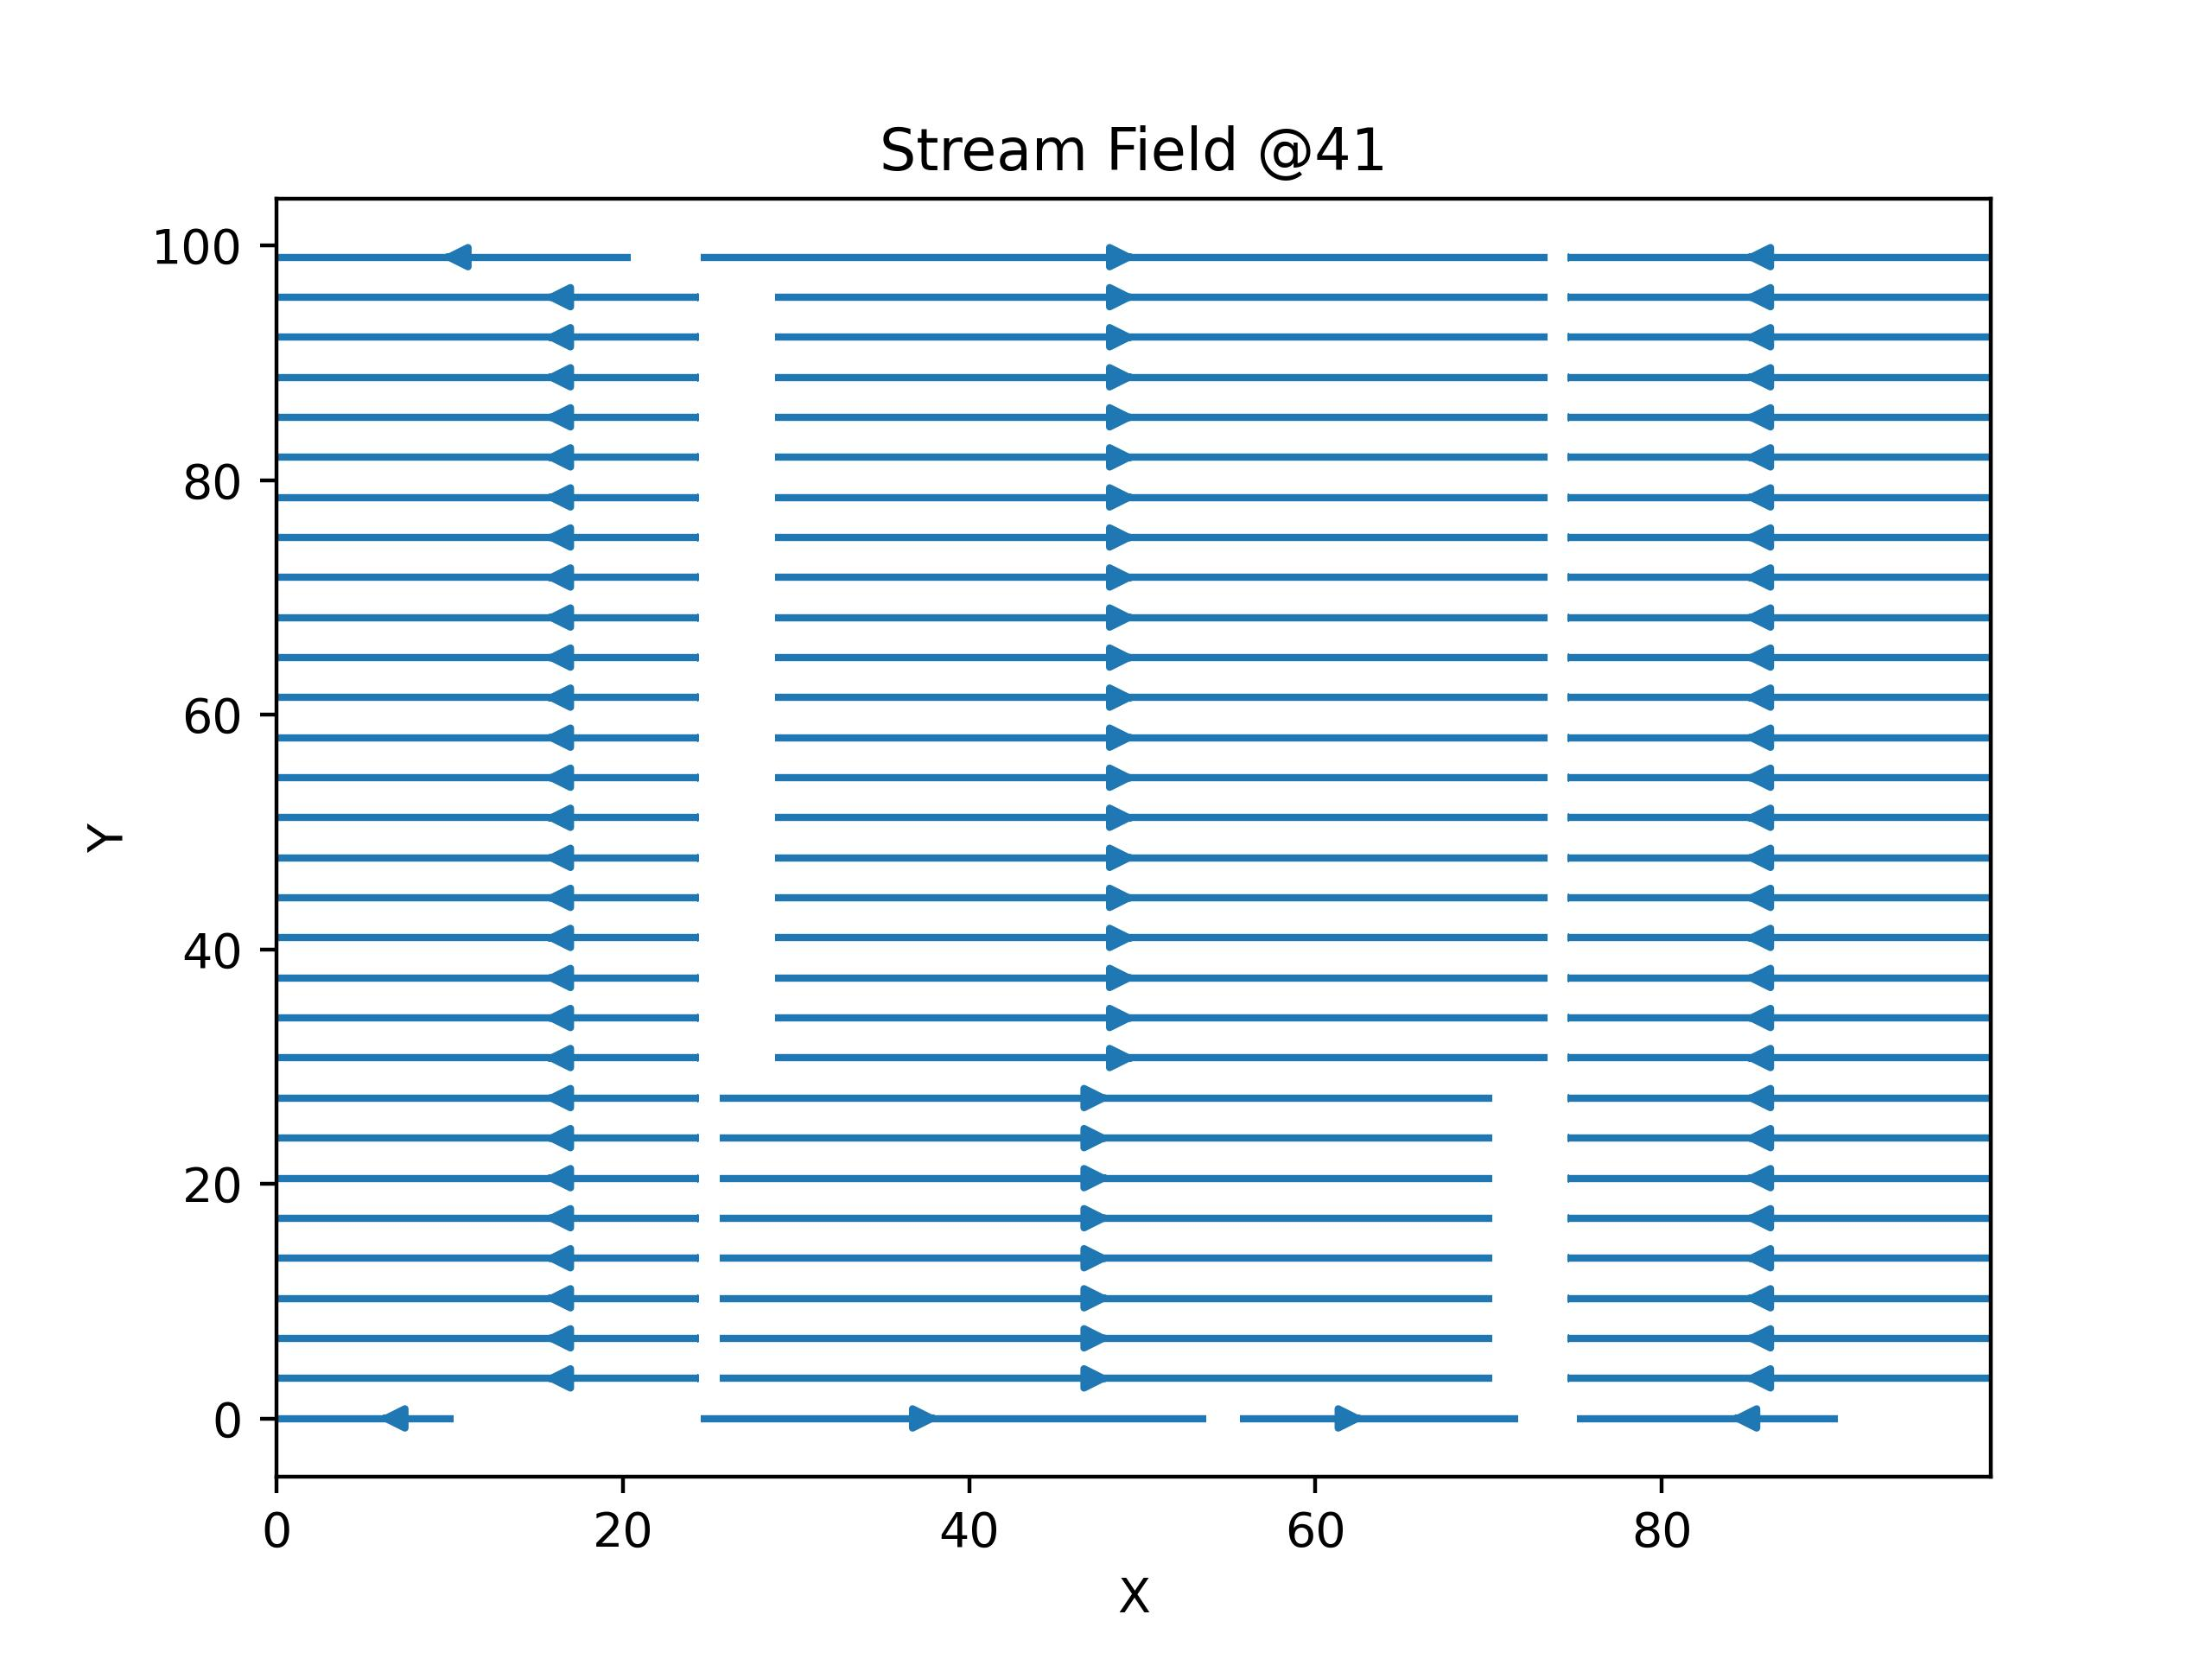
\includegraphics[width=\linewidth]{graphs/ShearWaveDecay/DensityDistribution/stream_field_41}
    \end{minipage}% don't remove this comment - uncomments a new line
    \begin{minipage}{0.33\textwidth}
        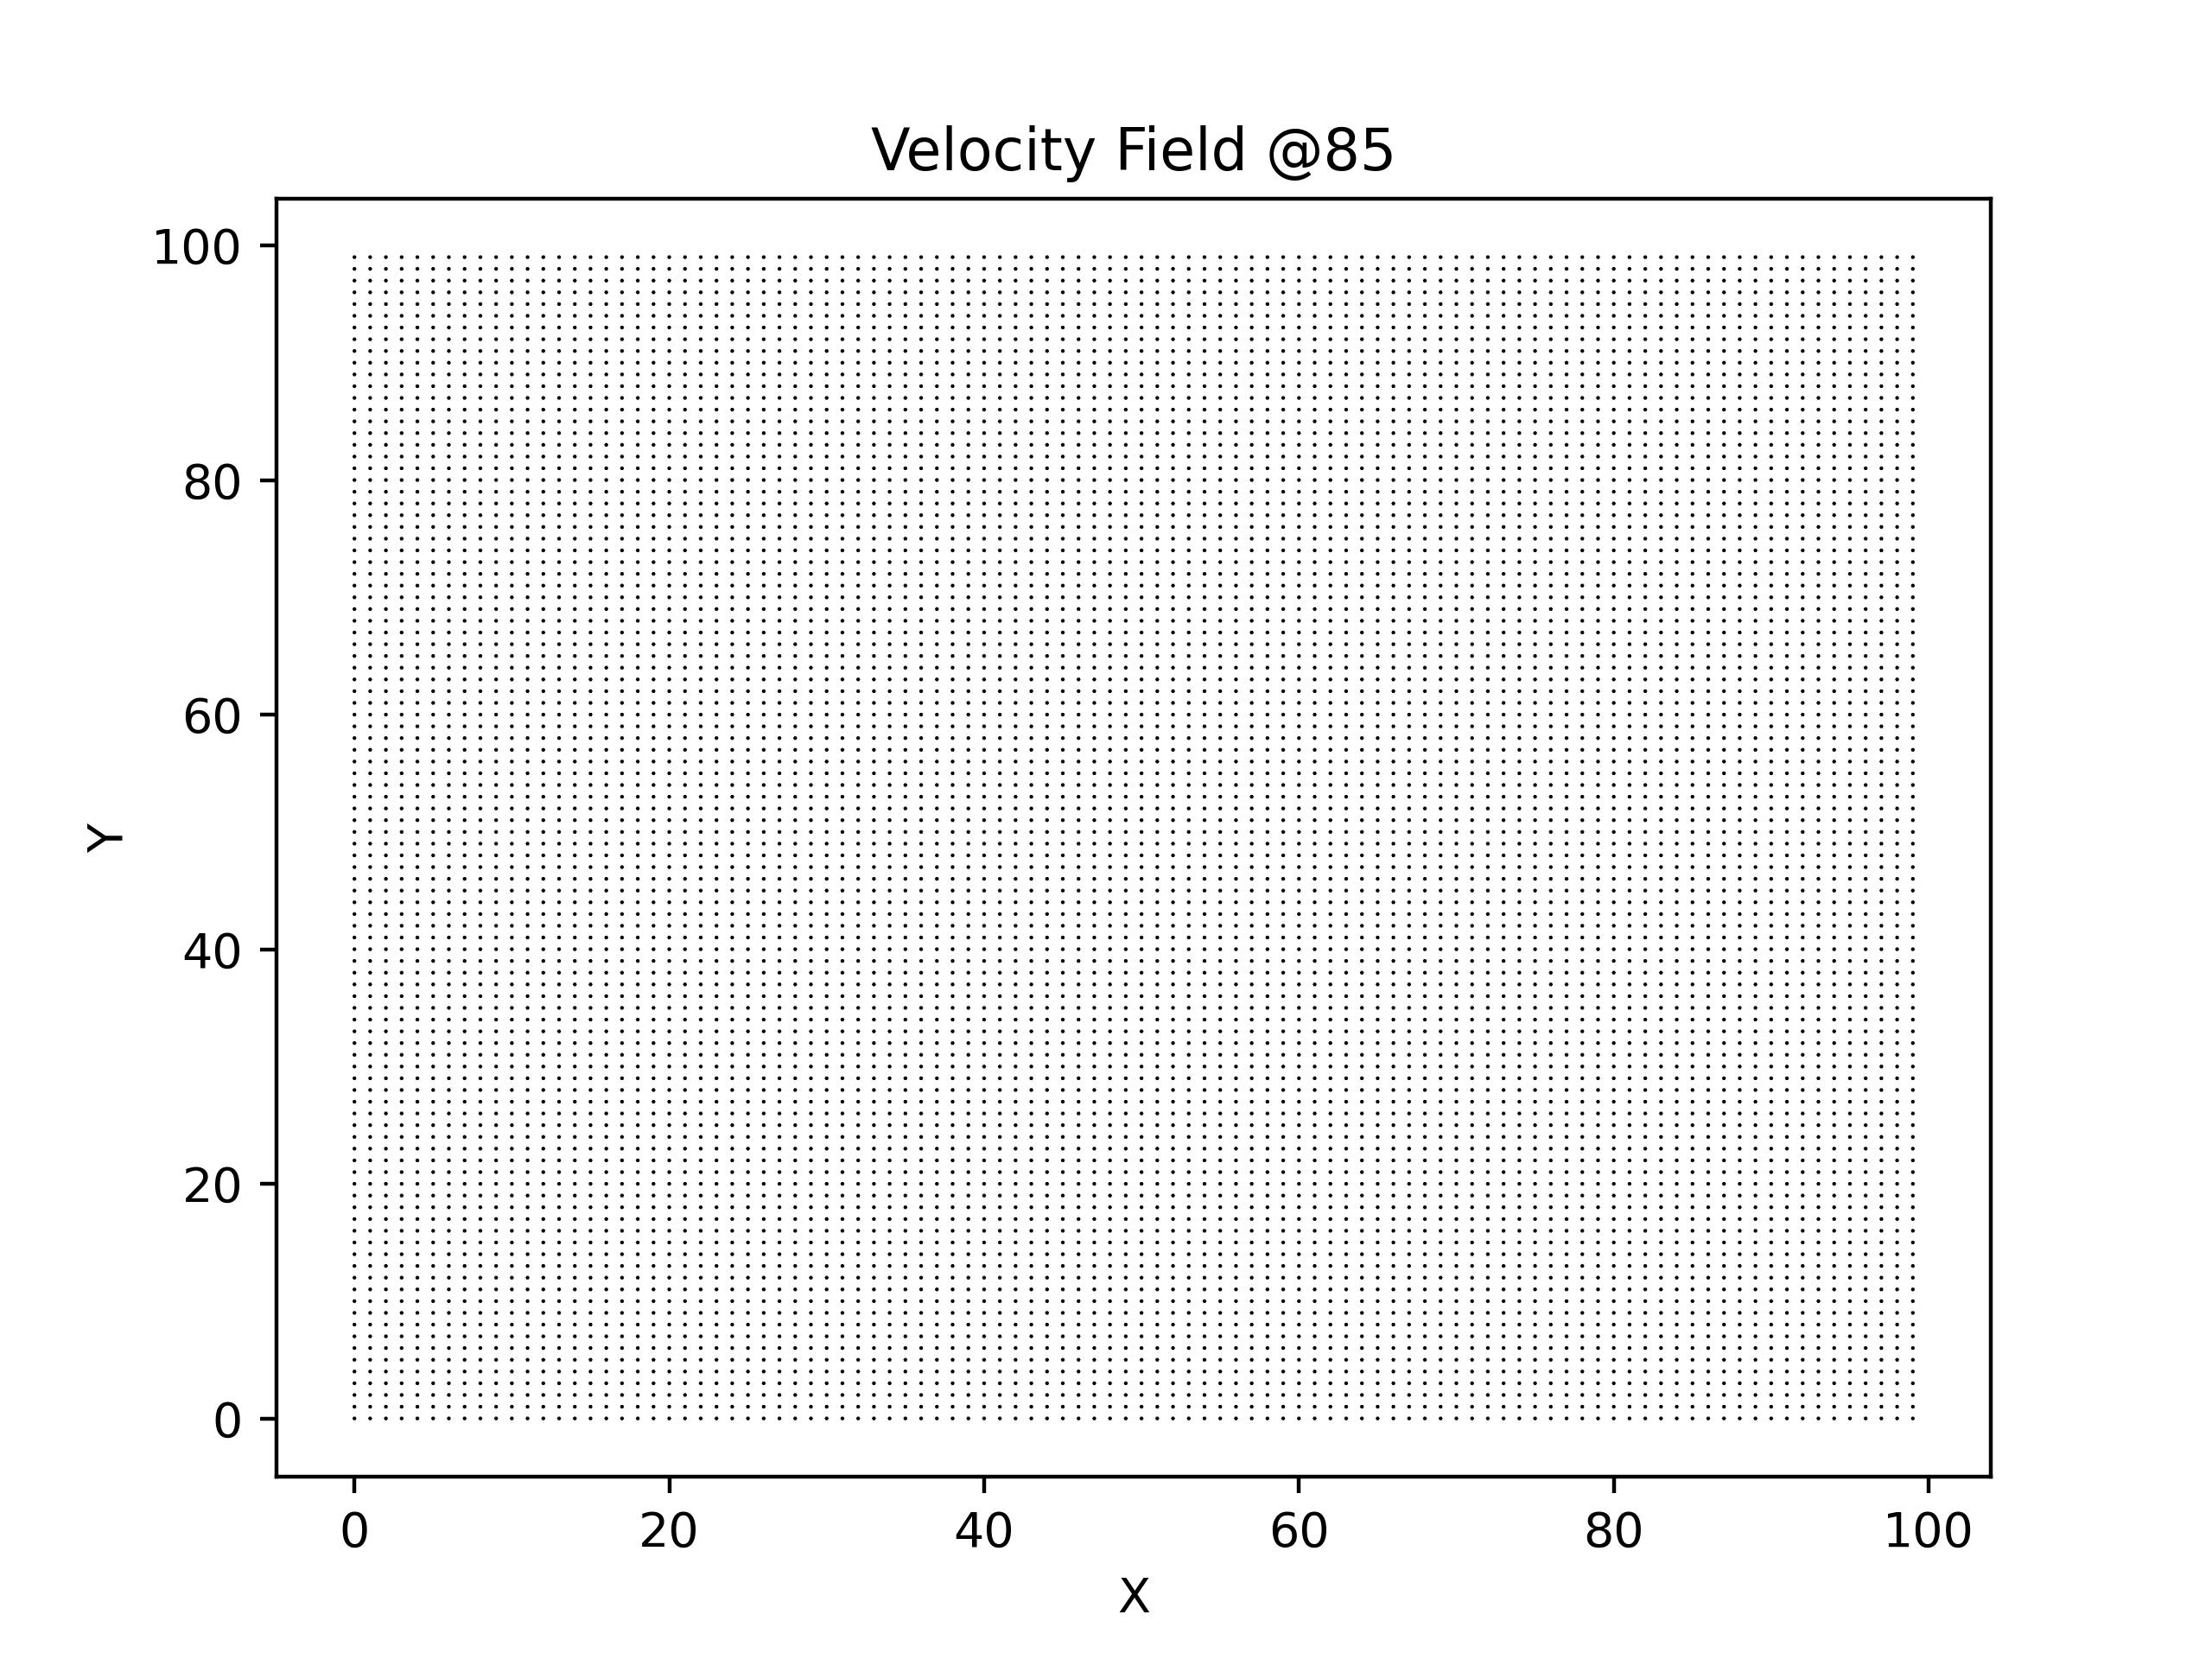
\includegraphics[width=\linewidth]{graphs/ShearWaveDecay/DensityDistribution/velocity_field_85}
    \end{minipage}% don't remove this comment - uncomments a new line
    \begin{minipage}{0.33\textwidth}
        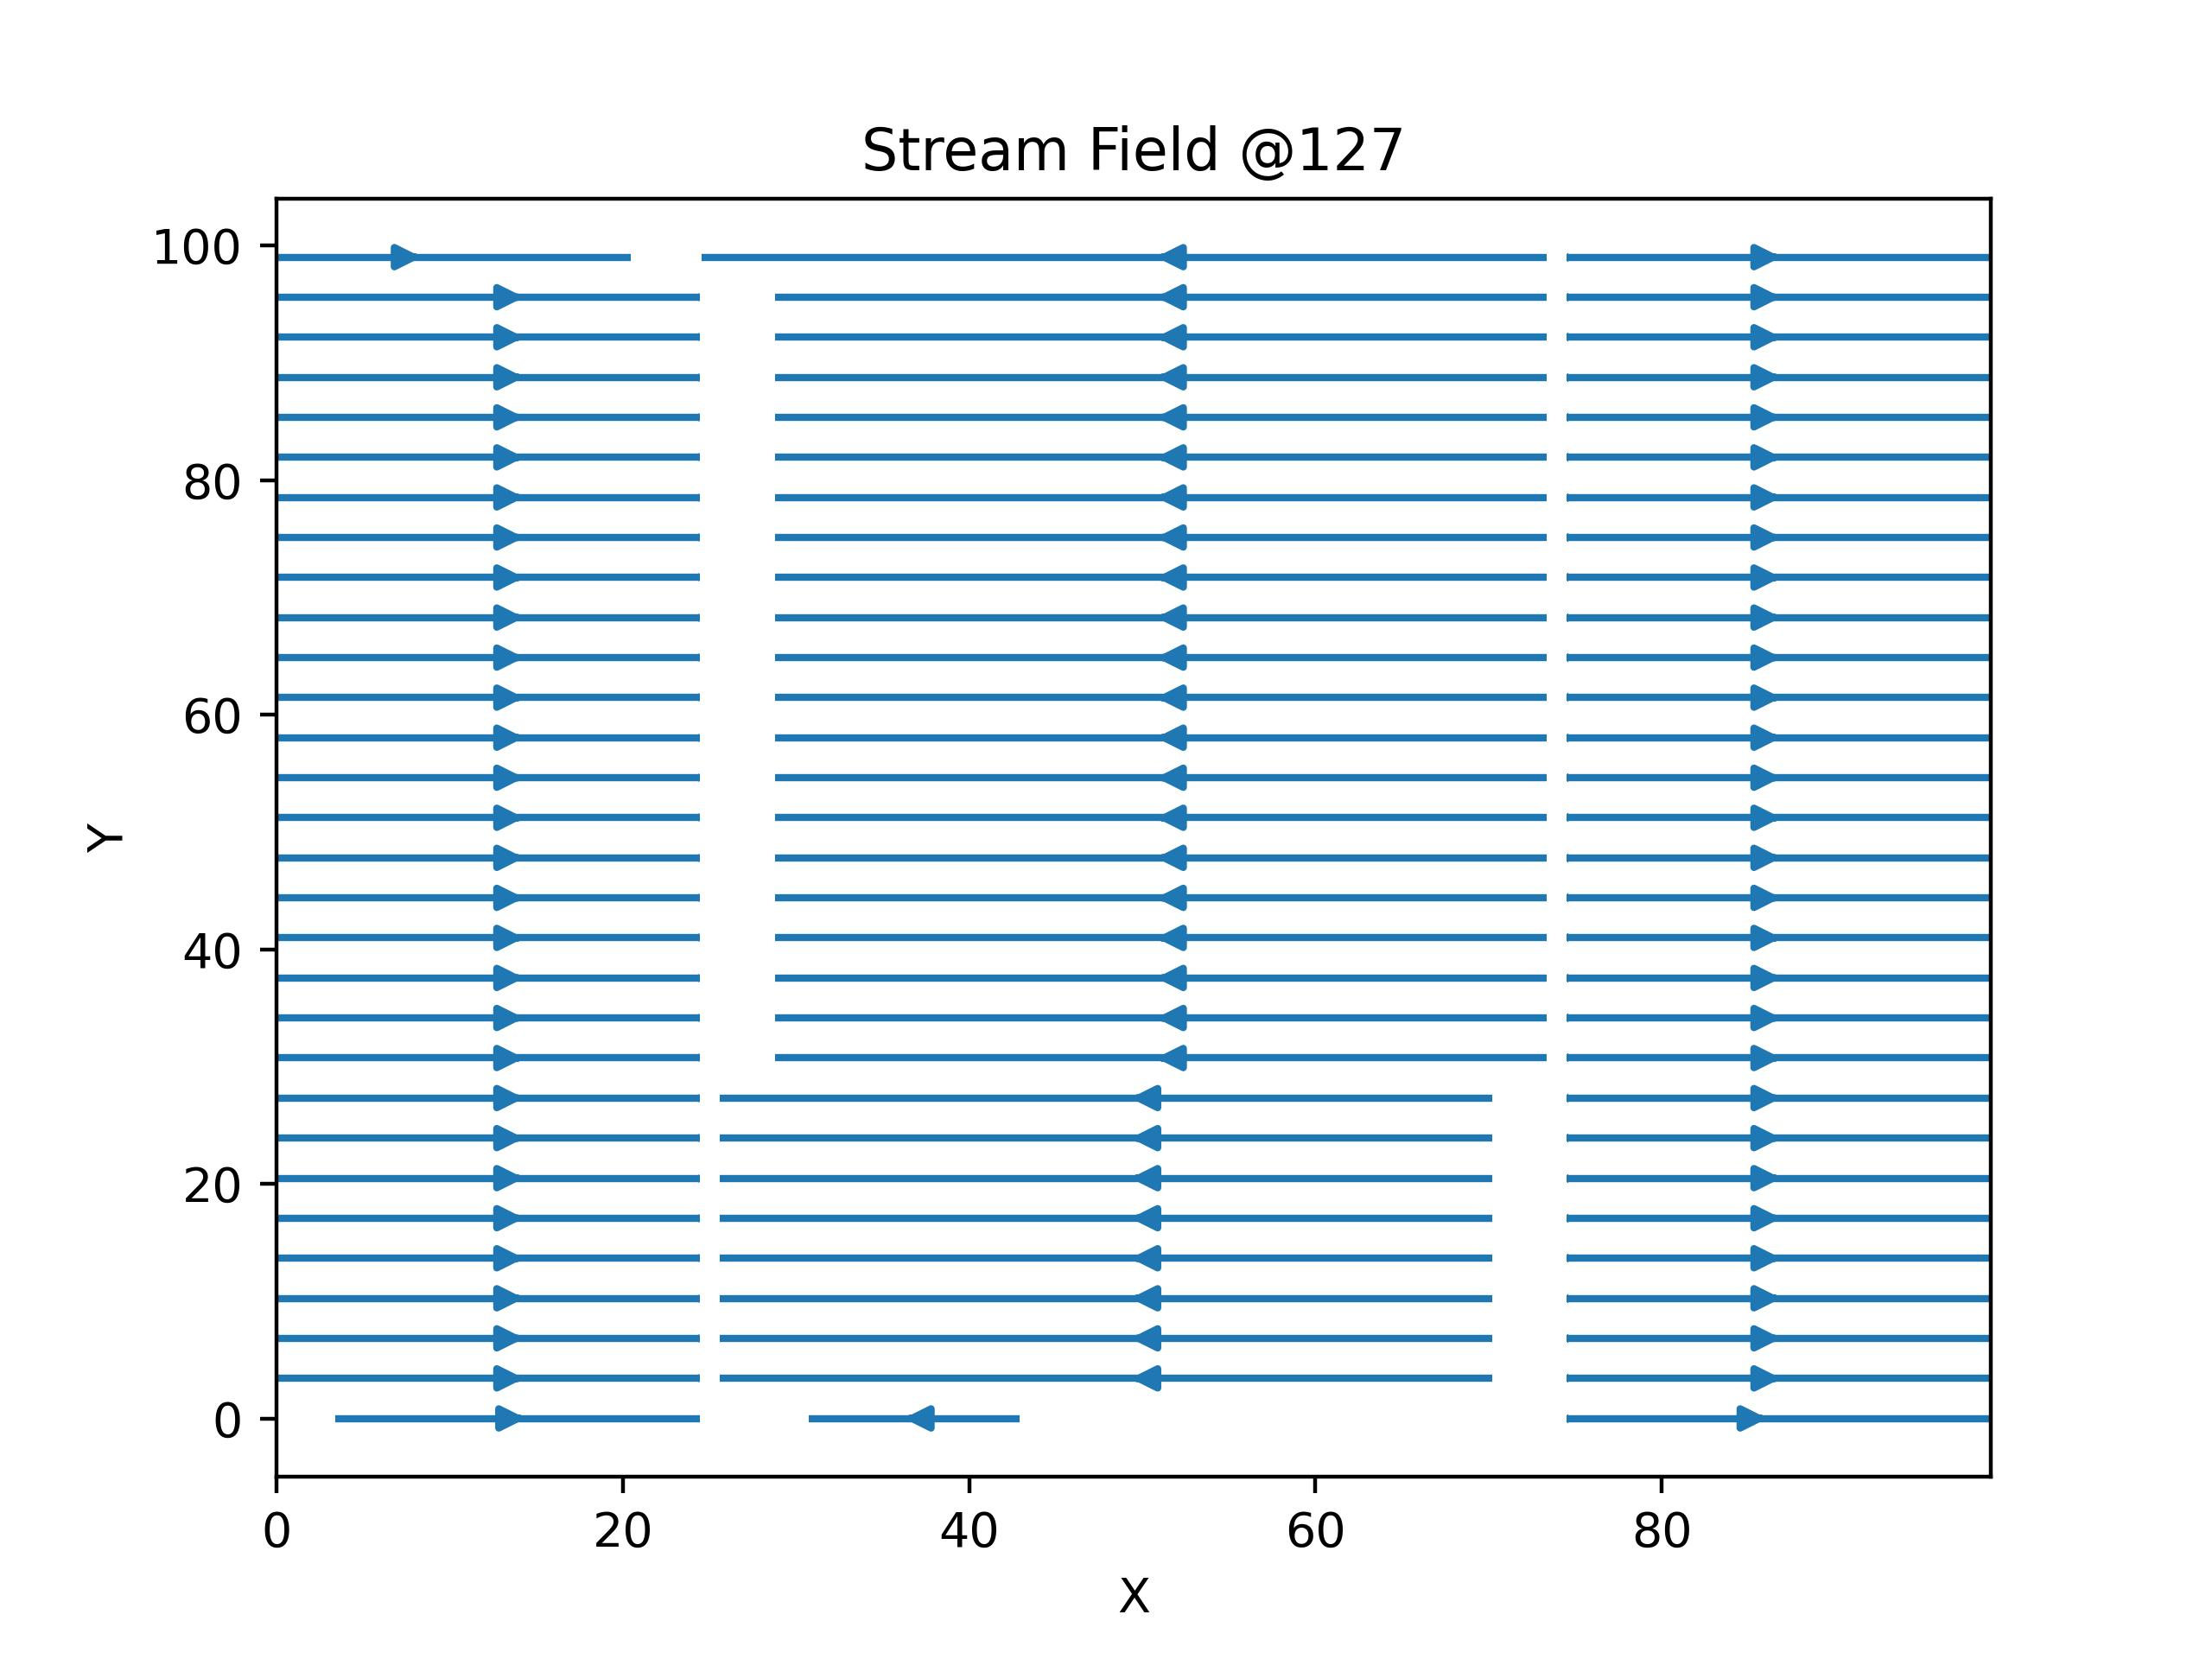
\includegraphics[width=\linewidth]{graphs/ShearWaveDecay/DensityDistribution/stream_field_127}
    \end{minipage}
    \caption{
        Different flow states during the simulation.
        From piling up at step 41 to a steady state at step 85 to the opposite flow at step 127.
    }
    \label{fig:swd-stream-velocity}
\end{figure}

This flow won't hold forever as the newly forming dense areas are always less dense as the once from the previous iteration.
The system tries to reach an equilibrium.
Over time the piles are shallower and shallower until it reaches the desired equilibrium function with the same density at all positions.
The decay is shown through the plots in \cref{fig:swd-decay}.

\begin{center}
    \begin{figure}[h!]
        \begin{minipage}{0.5\textwidth}
            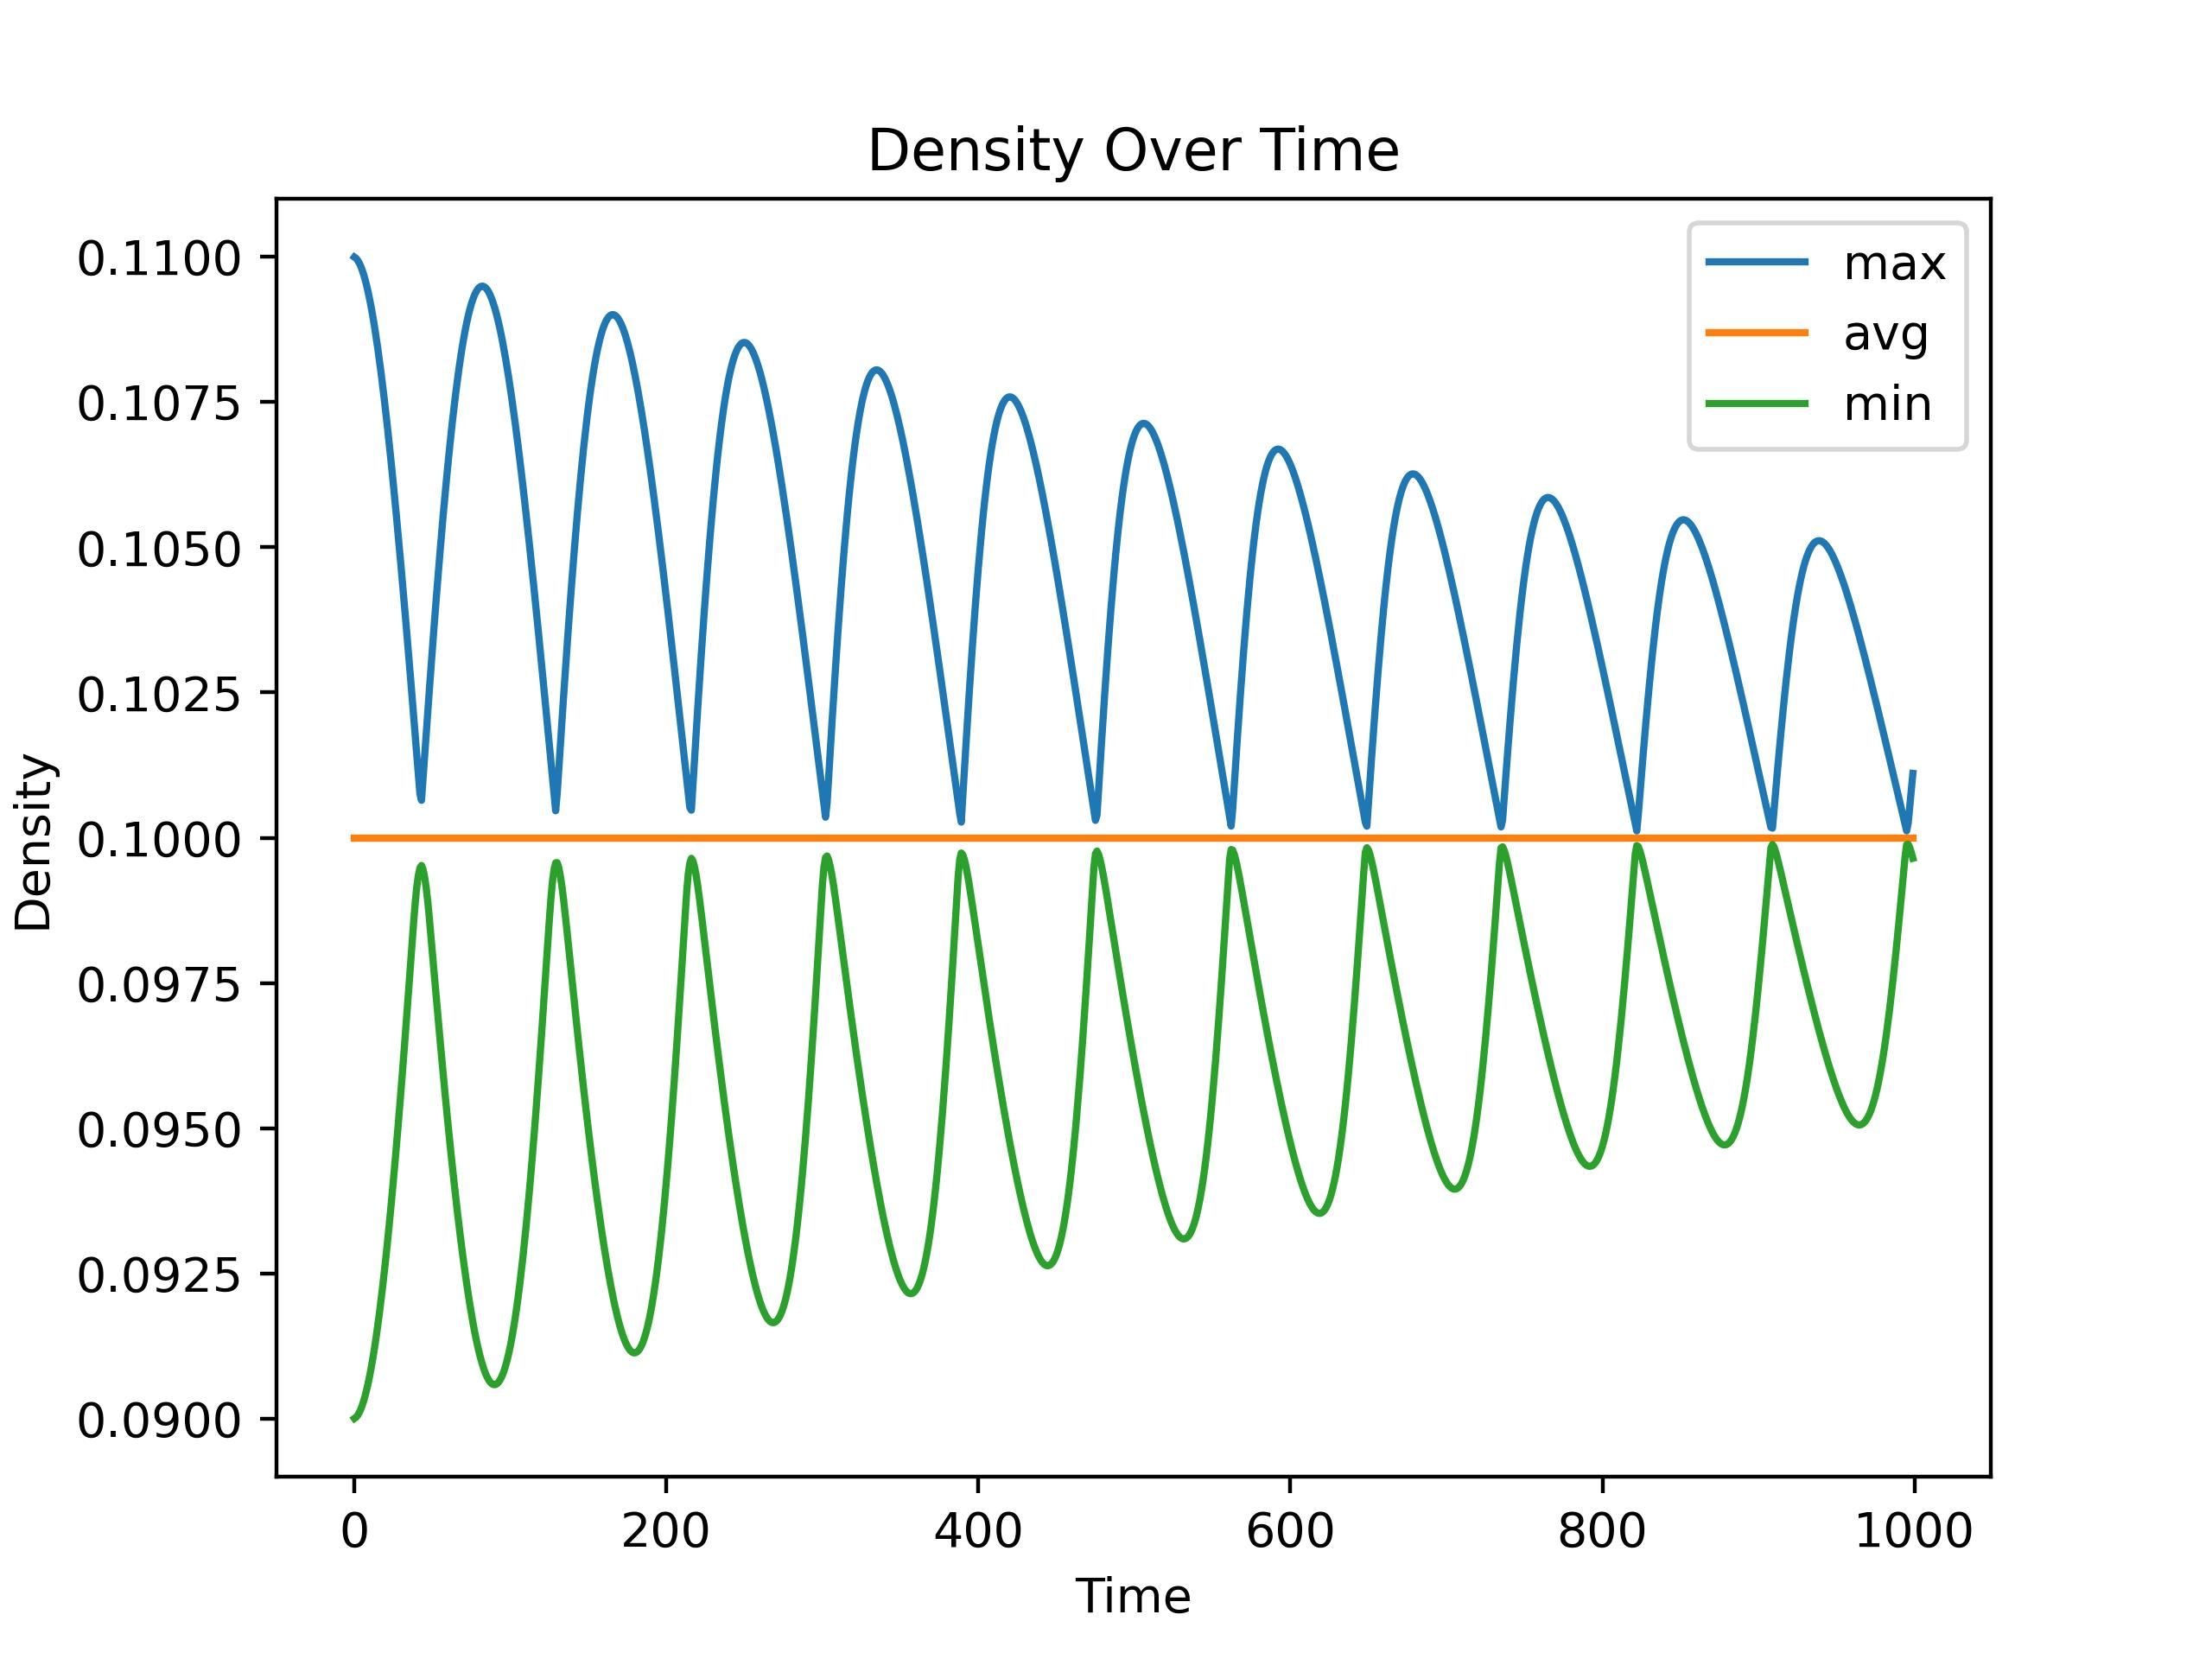
\includegraphics[width=\linewidth]{graphs/ShearWaveDecay/DensityDistribution/density_aggregate_over_time.jpg}
        \end{minipage}% don't remove this comment - uncomments a new line
        \begin{minipage}{0.5\textwidth}
            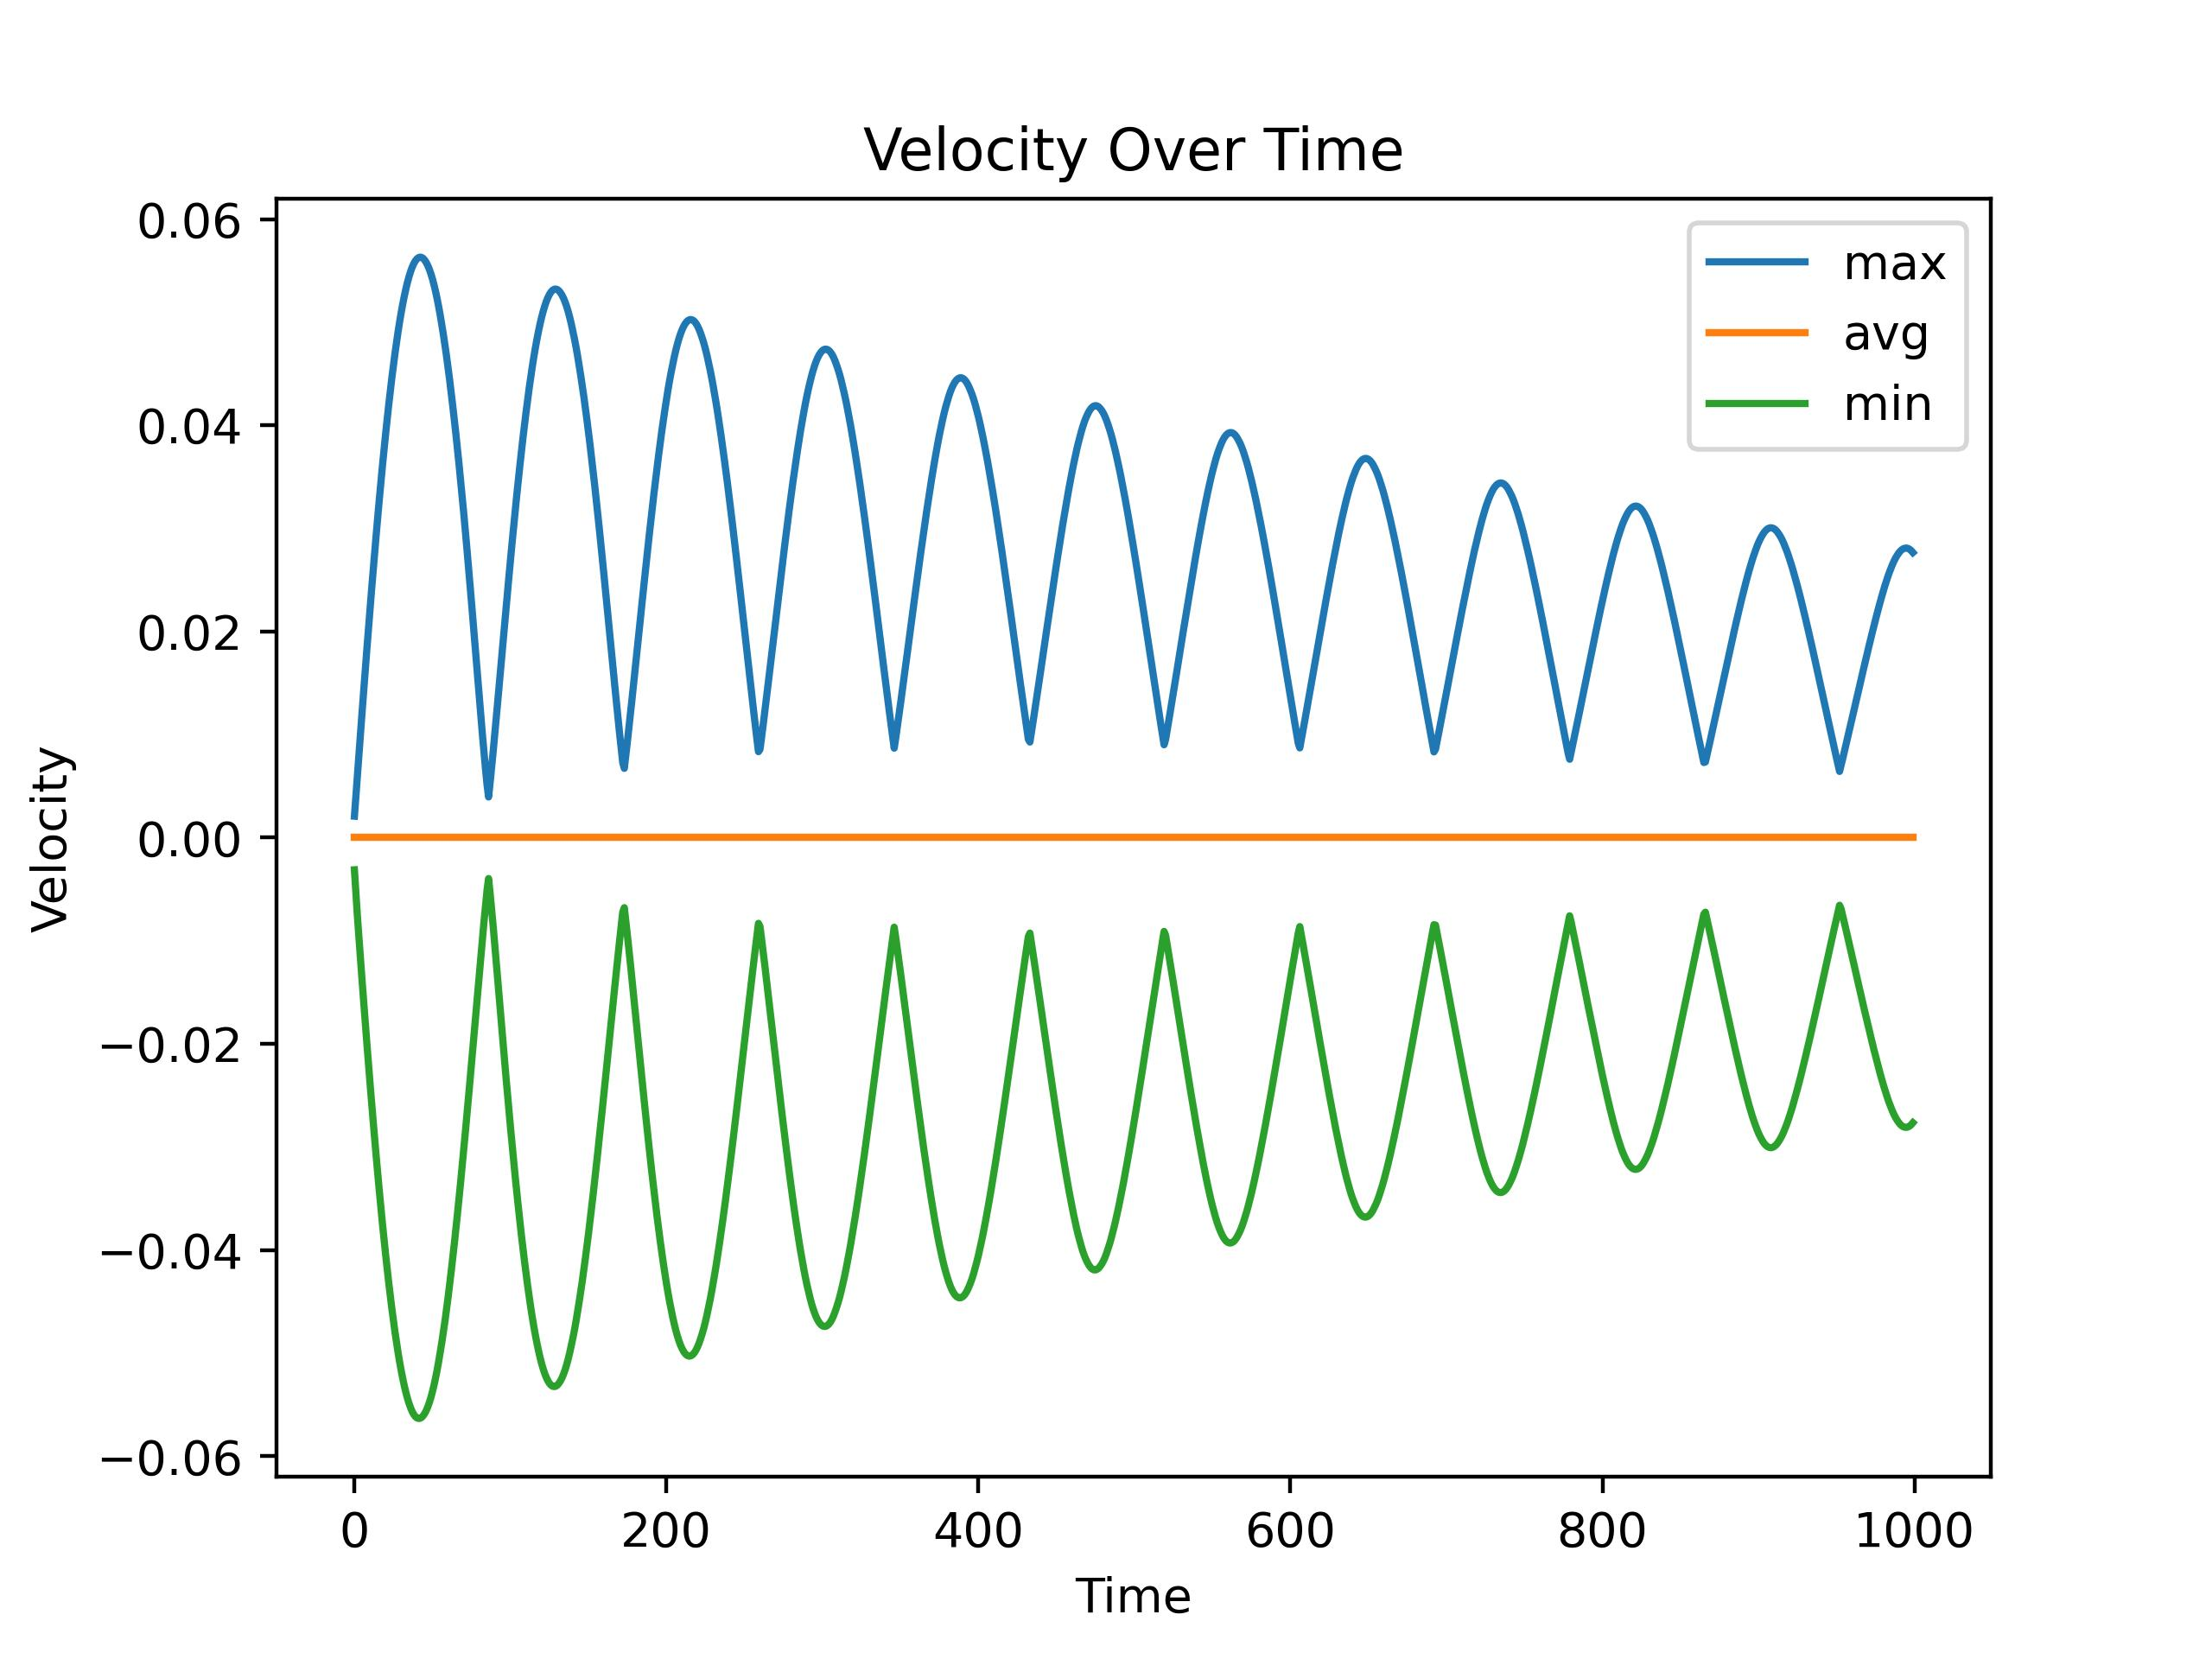
\includegraphics[width=\linewidth]{graphs/ShearWaveDecay/DensityDistribution/velocity_aggregate_over_time.jpg}
        \end{minipage}
        \caption{Decaying density and velocity over time.}
        \label{fig:swd-decay}
    \end{figure}
\end{center}

\subsection{Sinusoidal Velocity}\label{subsec:sinusoidal-velocity}
\textbf{This experiment ran with an epsilon of 0.5 to display the effect more drastically.}
The initial condition is a given by the following equation where $L_y$ resembles the size in y-direction and $\epsilon$ resembles the initial amplitude

\begin{equation*}
    \begin{aligned}
        u_x(\mathbf{r},0) &= \epsilon \sin \left( \frac{2 \pi x}{L_y} \right) \\
        \rho(\mathbf{r},0) &= 1 \cdot
    \end{aligned}
\end{equation*}

Because of the initial condition, the flow varies throughout the field.
The equilibrium state is a state without a clearly directed movement as in the initial condition.
So it is expected that the flow will decrease over time.

\begin{figure}[h!]
    \begin{minipage}{0.33\textwidth}
        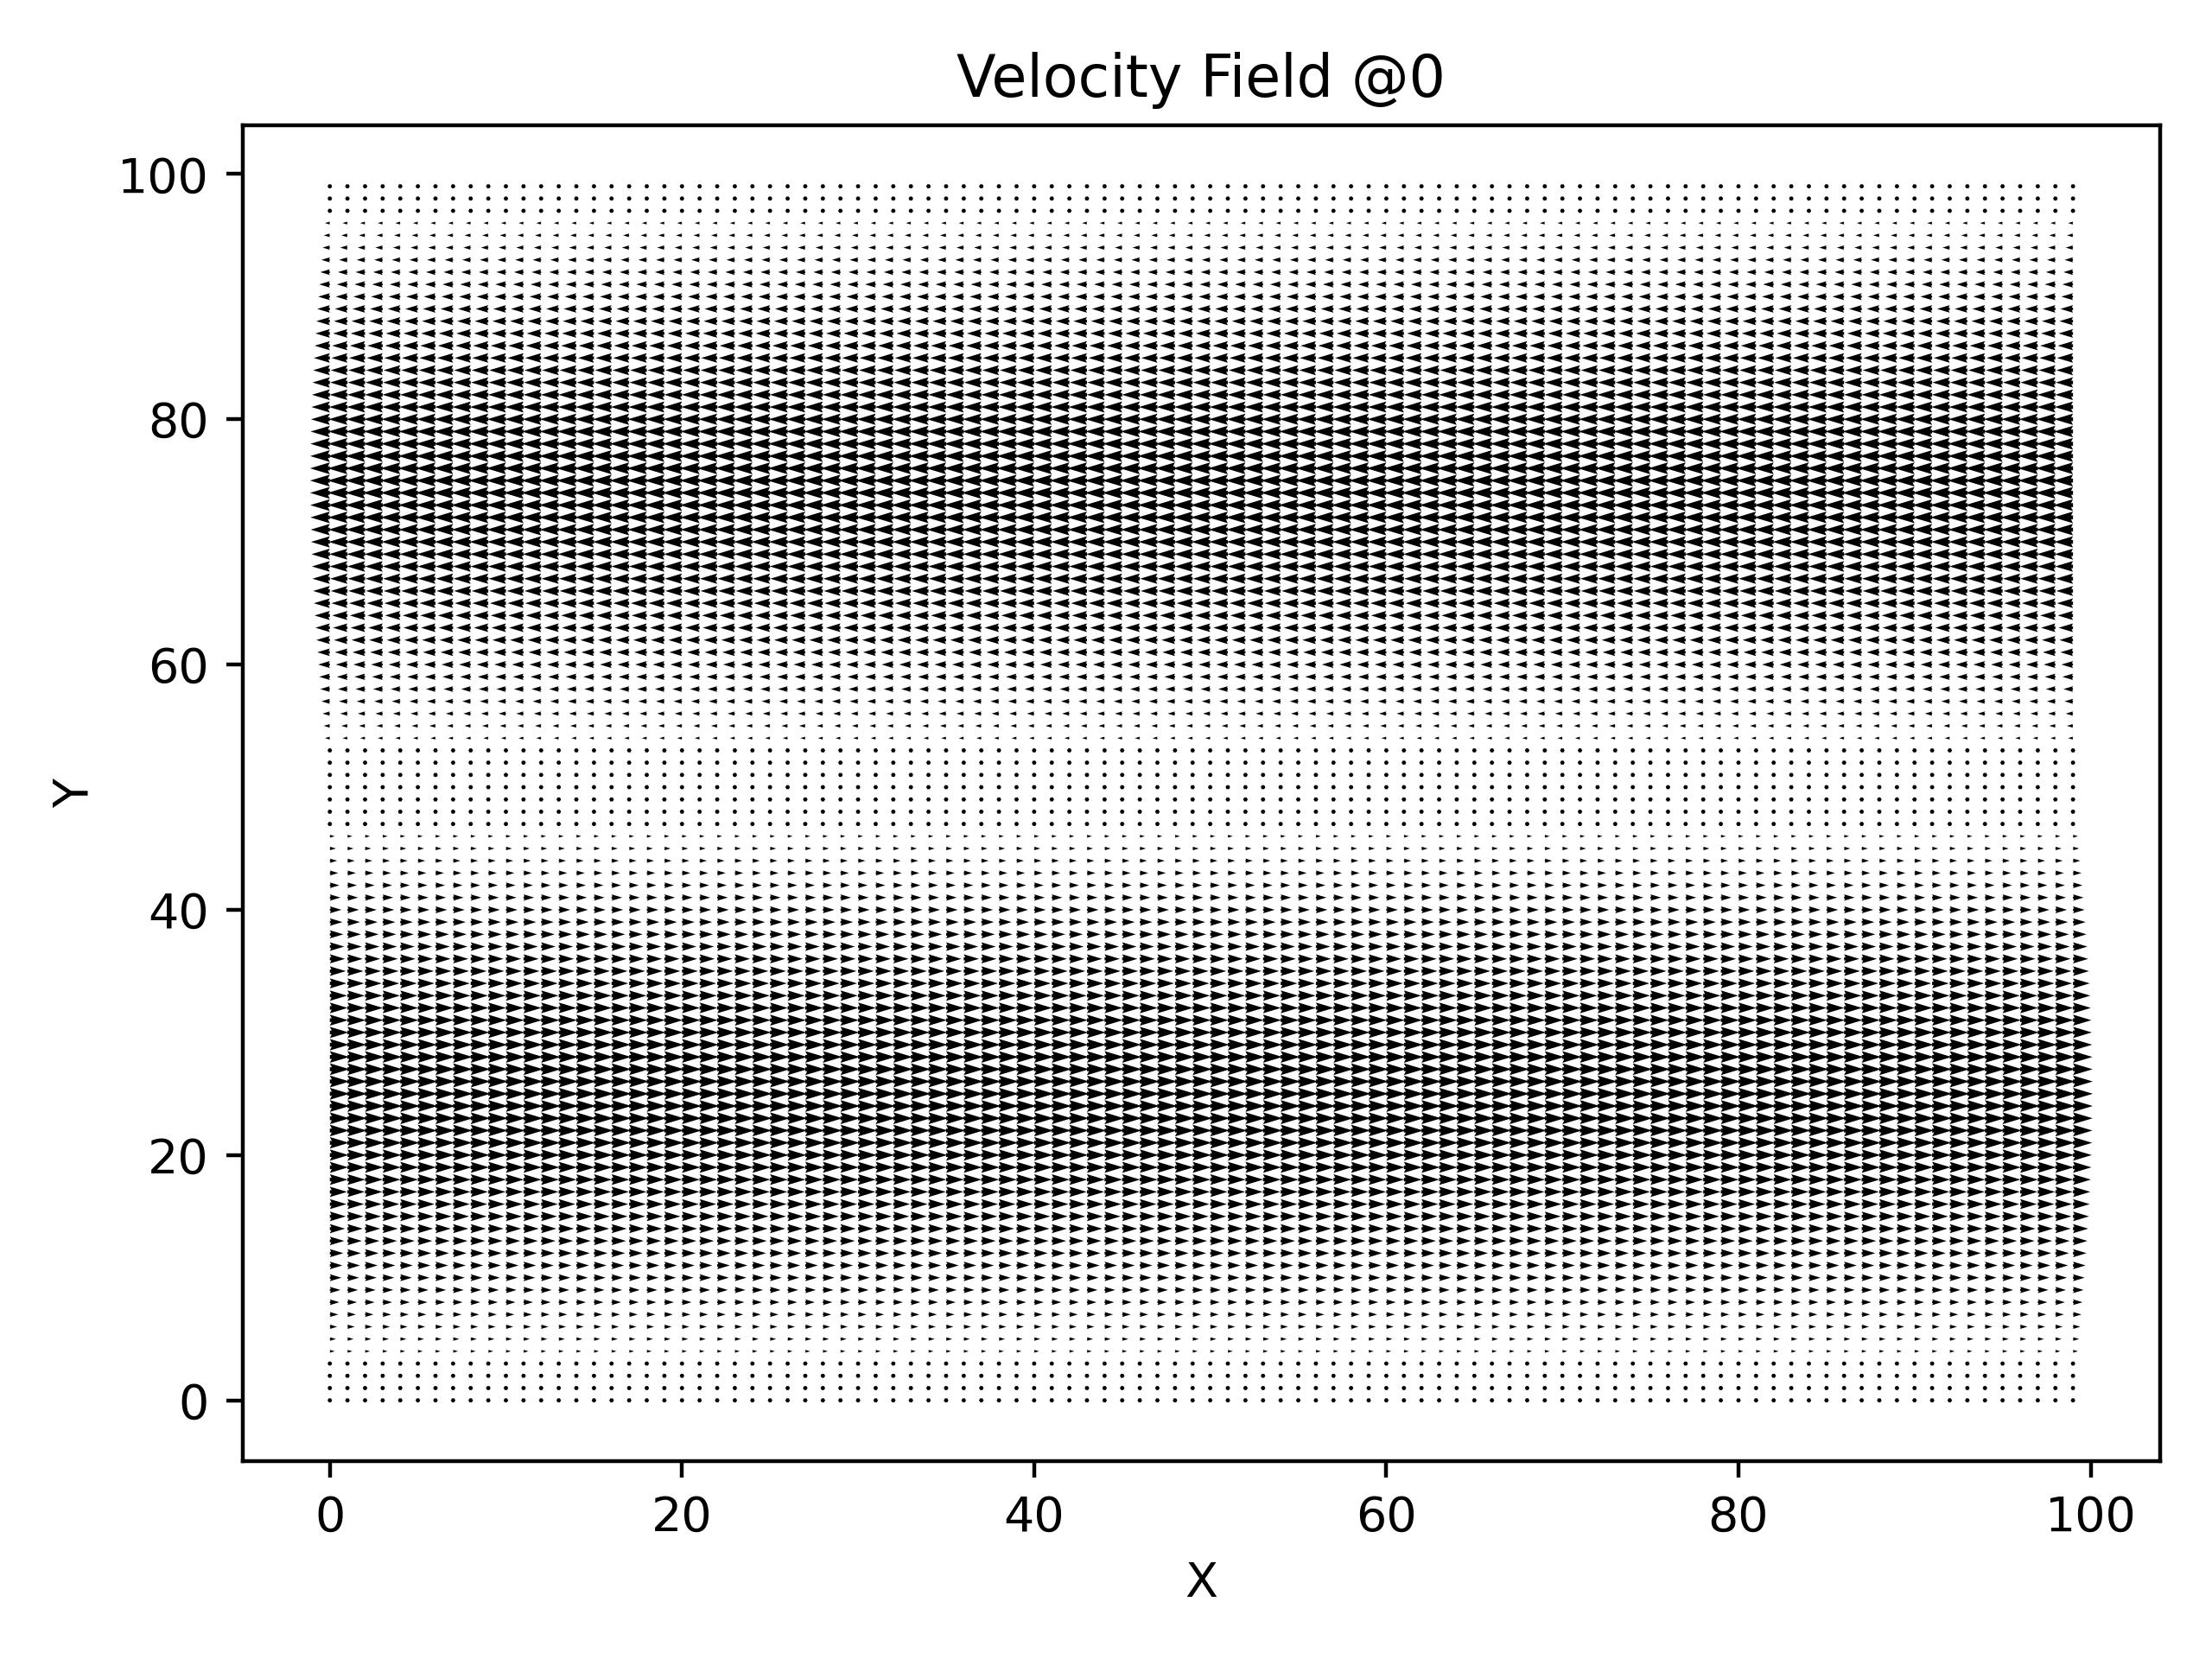
\includegraphics[width=\linewidth]{graphs/ShearWaveDecay/VelocityDistribution/velocity_field_0}
    \end{minipage}% don't remove this comment - uncomments a new line
    \begin{minipage}{0.33\textwidth}
        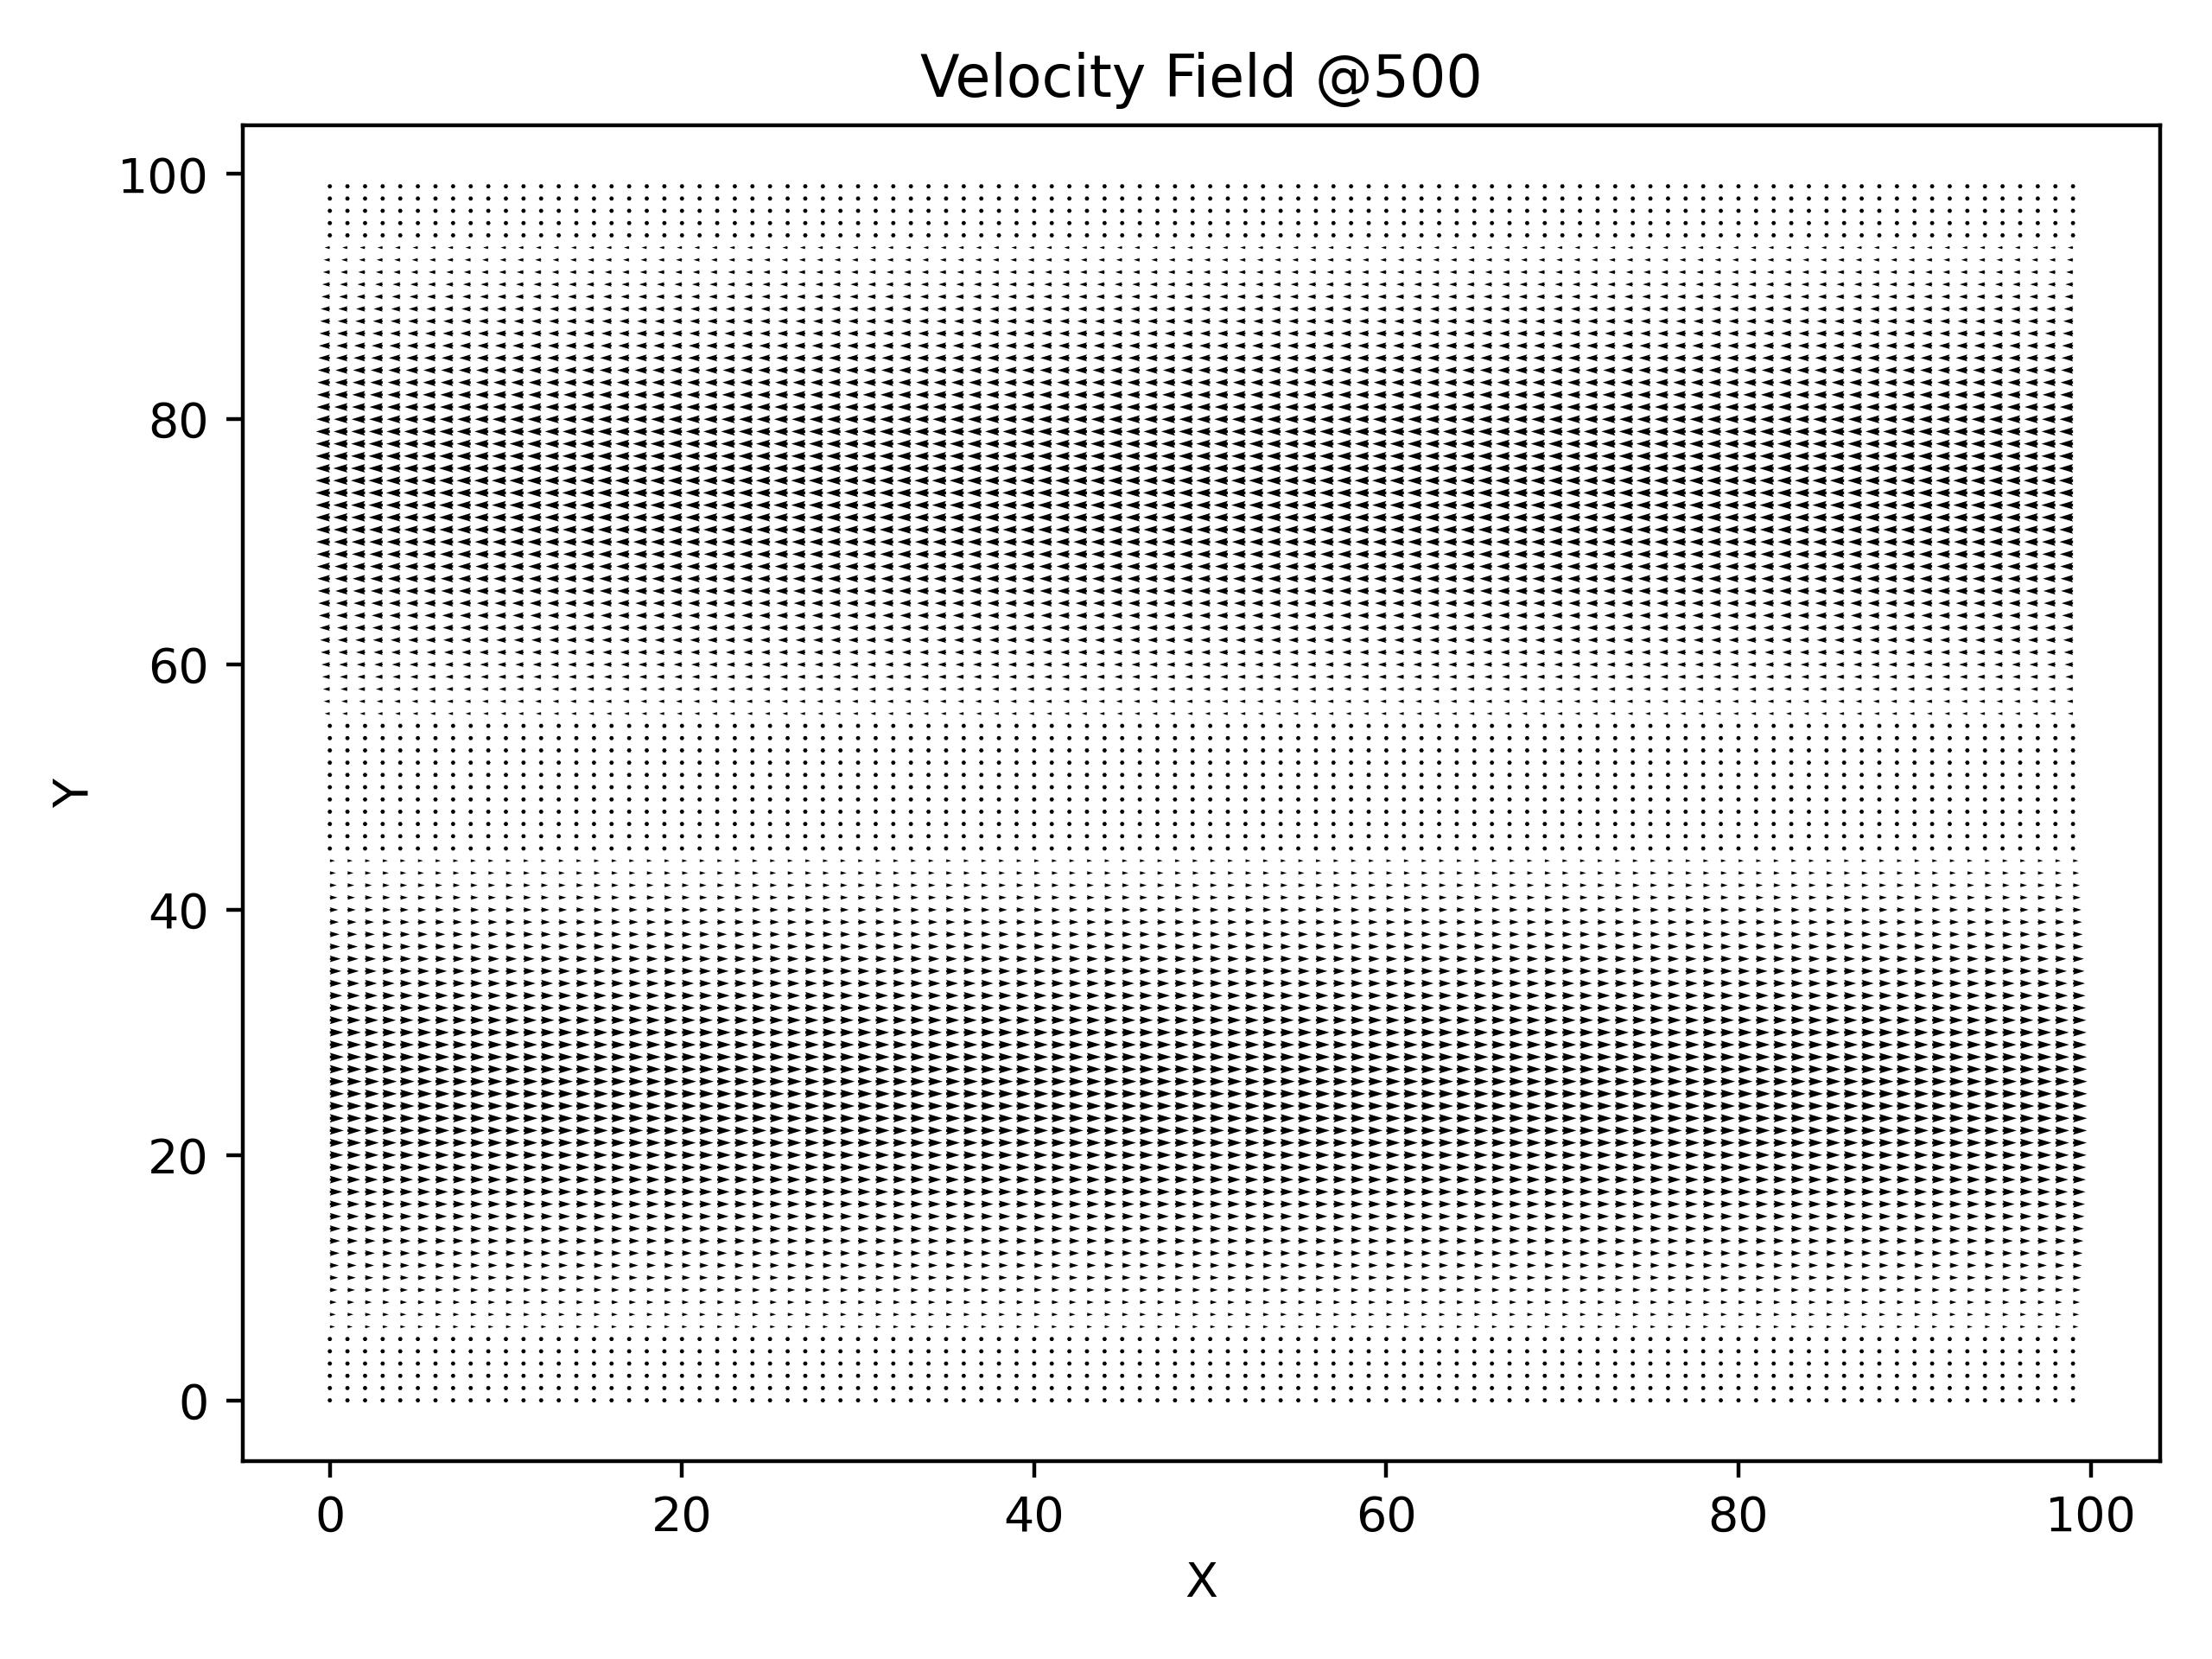
\includegraphics[width=\linewidth]{graphs/ShearWaveDecay/VelocityDistribution/velocity_field_500}
    \end{minipage}% don't remove this comment - uncomments a new line
    \begin{minipage}{0.33\textwidth}
        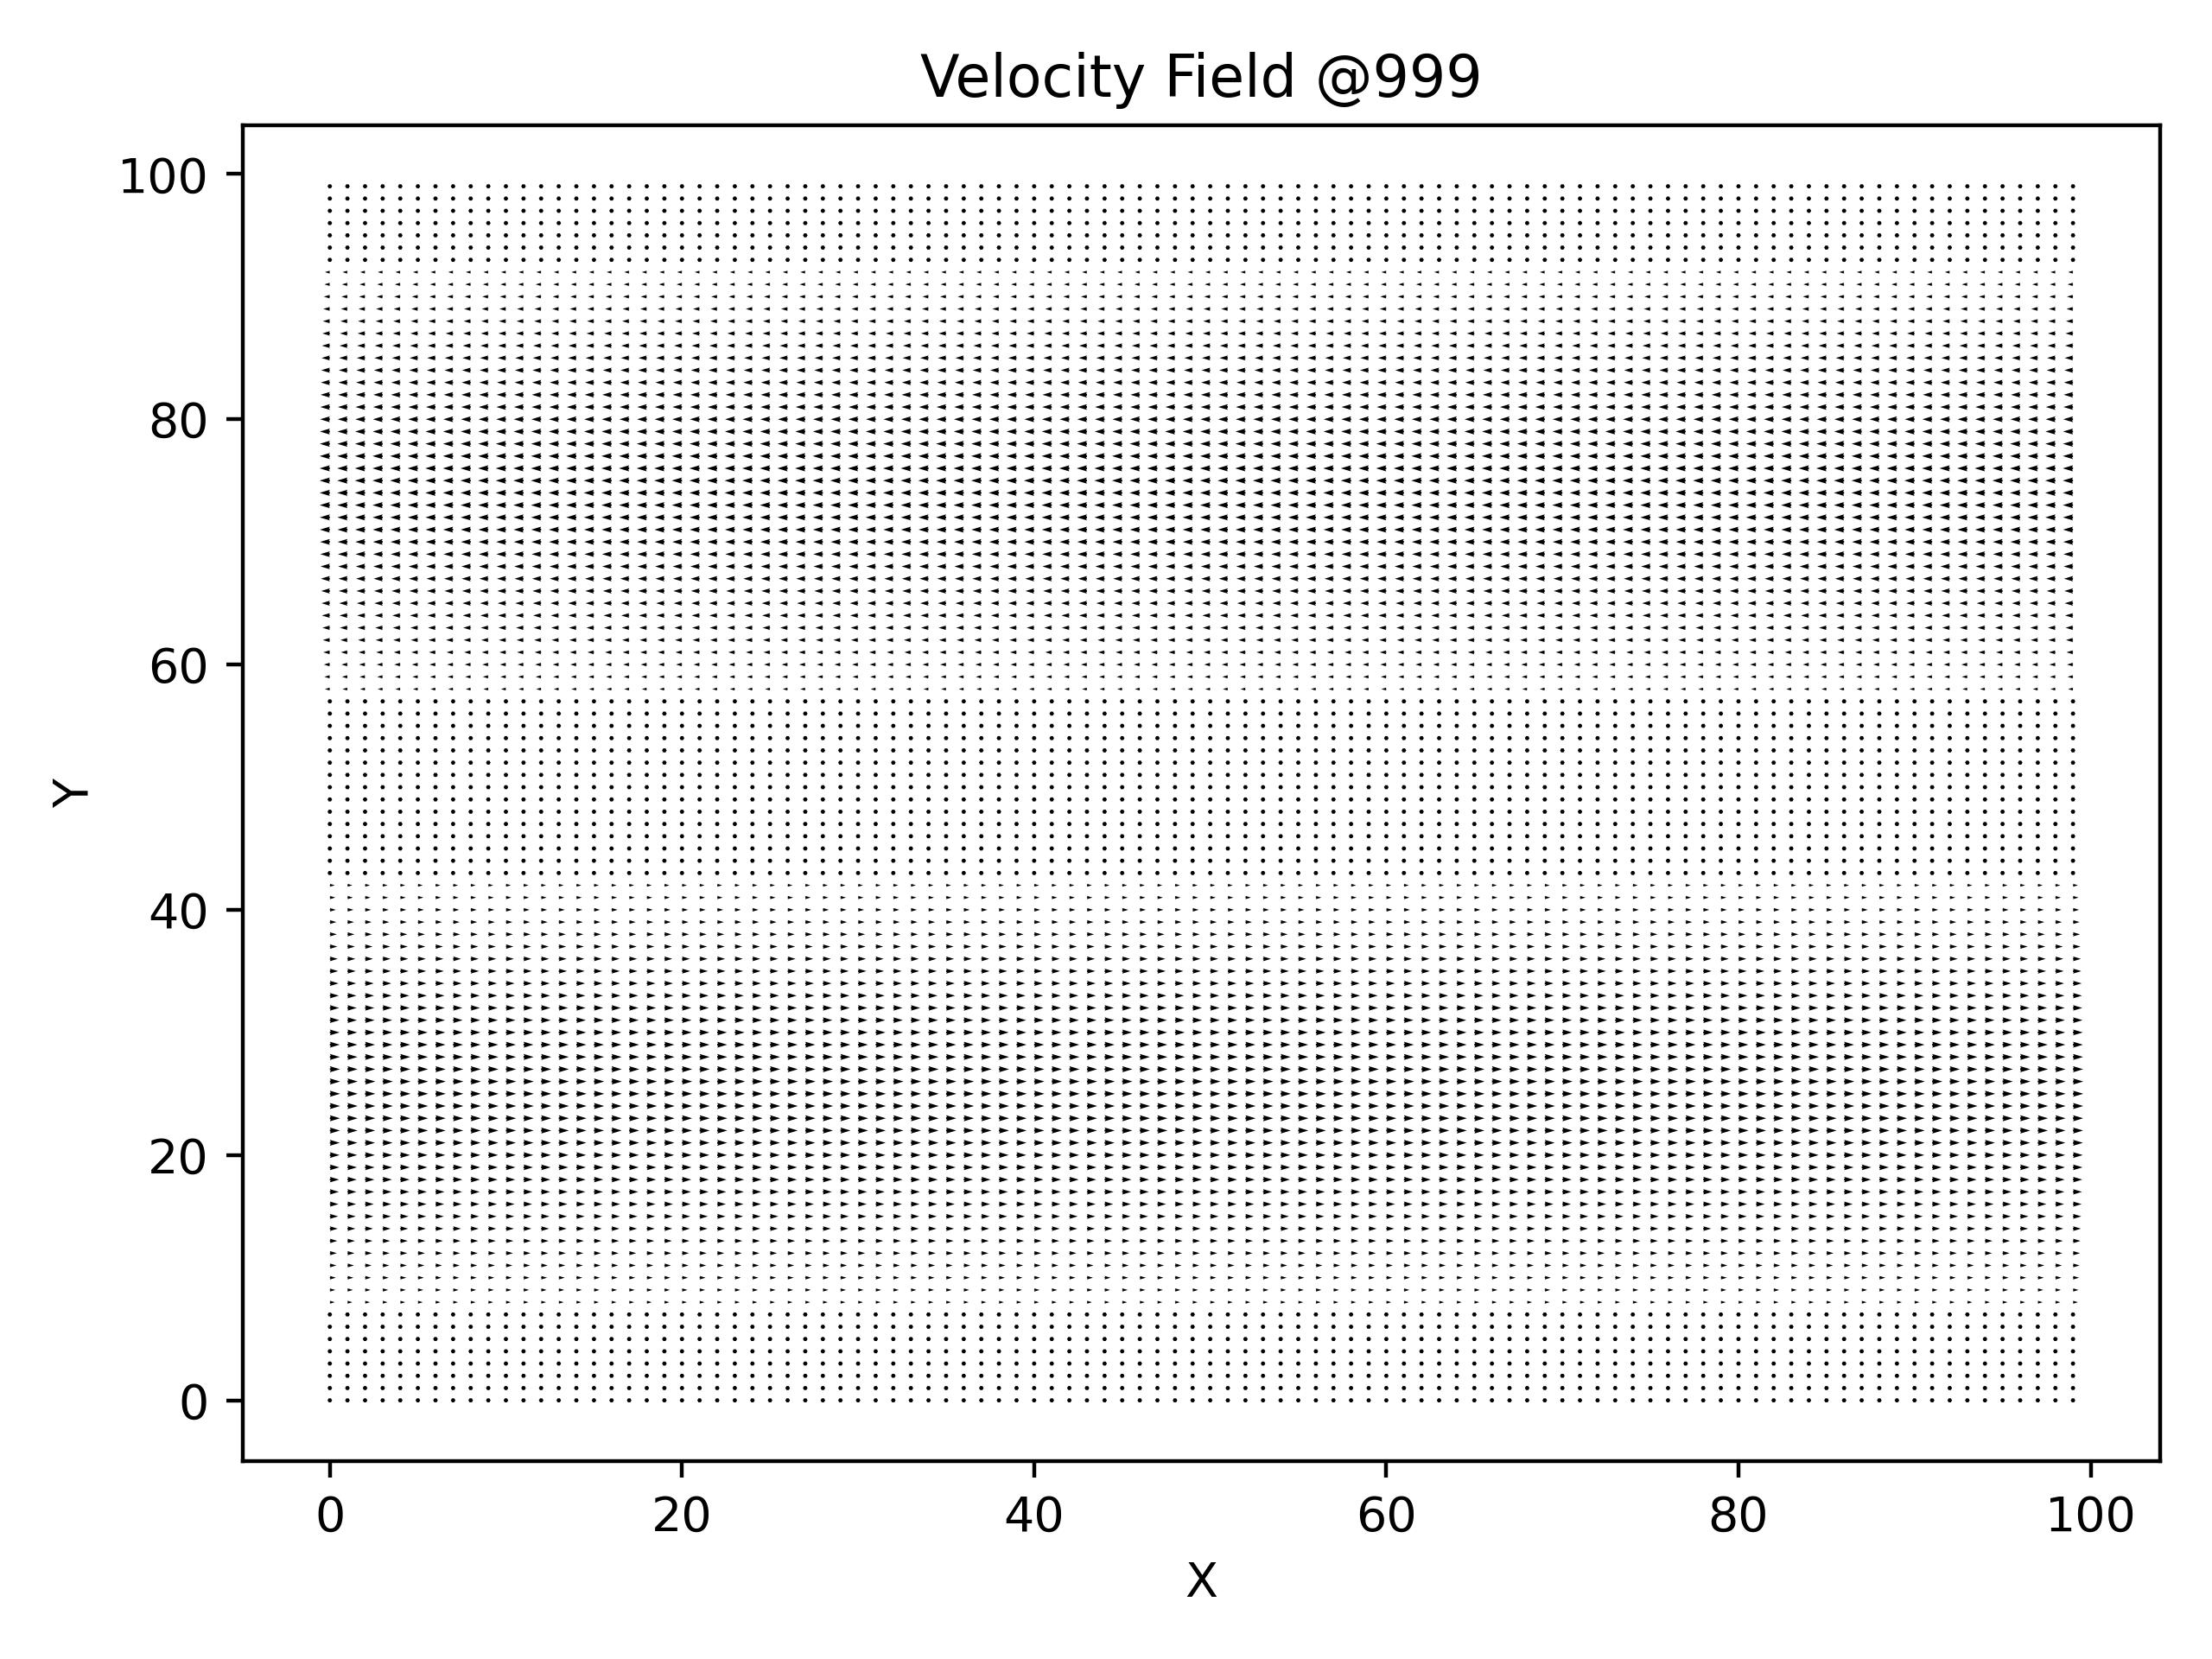
\includegraphics[width=\linewidth]{graphs/ShearWaveDecay/VelocityDistribution/velocity_field_999}
    \end{minipage}
    \caption{
        Different flow states during the simulation.
        From the sinusoid initial condition with a steady decrease till step 999.
    }
    \label{fig:swd-vs-velocity-fields}
\end{figure}

\Cref{fig:swd-vs-velocity-fields} gives a brief overview over the initial flow, and it's decaying over time.
While at step 0, a strong sinusoid flow can be seen, at timestep 999 it decreased visibly.
This decrease can be even further shown in \cref{fig:swd-vs-at-column_x} which shows the decay at a specific column.
The decay rate is also in line with the theoretical solution (as seen in \cref{fig:swd-vs-ideal}) given by
\begin{equation*}
    \begin{aligned}
        a_t &= a_0 e^{-vt \frac{2\pi}{L_y}^2}
    \end{aligned}
\end{equation*}

\begin{center}
    \begin{figure}[h!]
        \begin{minipage}{0.5\textwidth}
            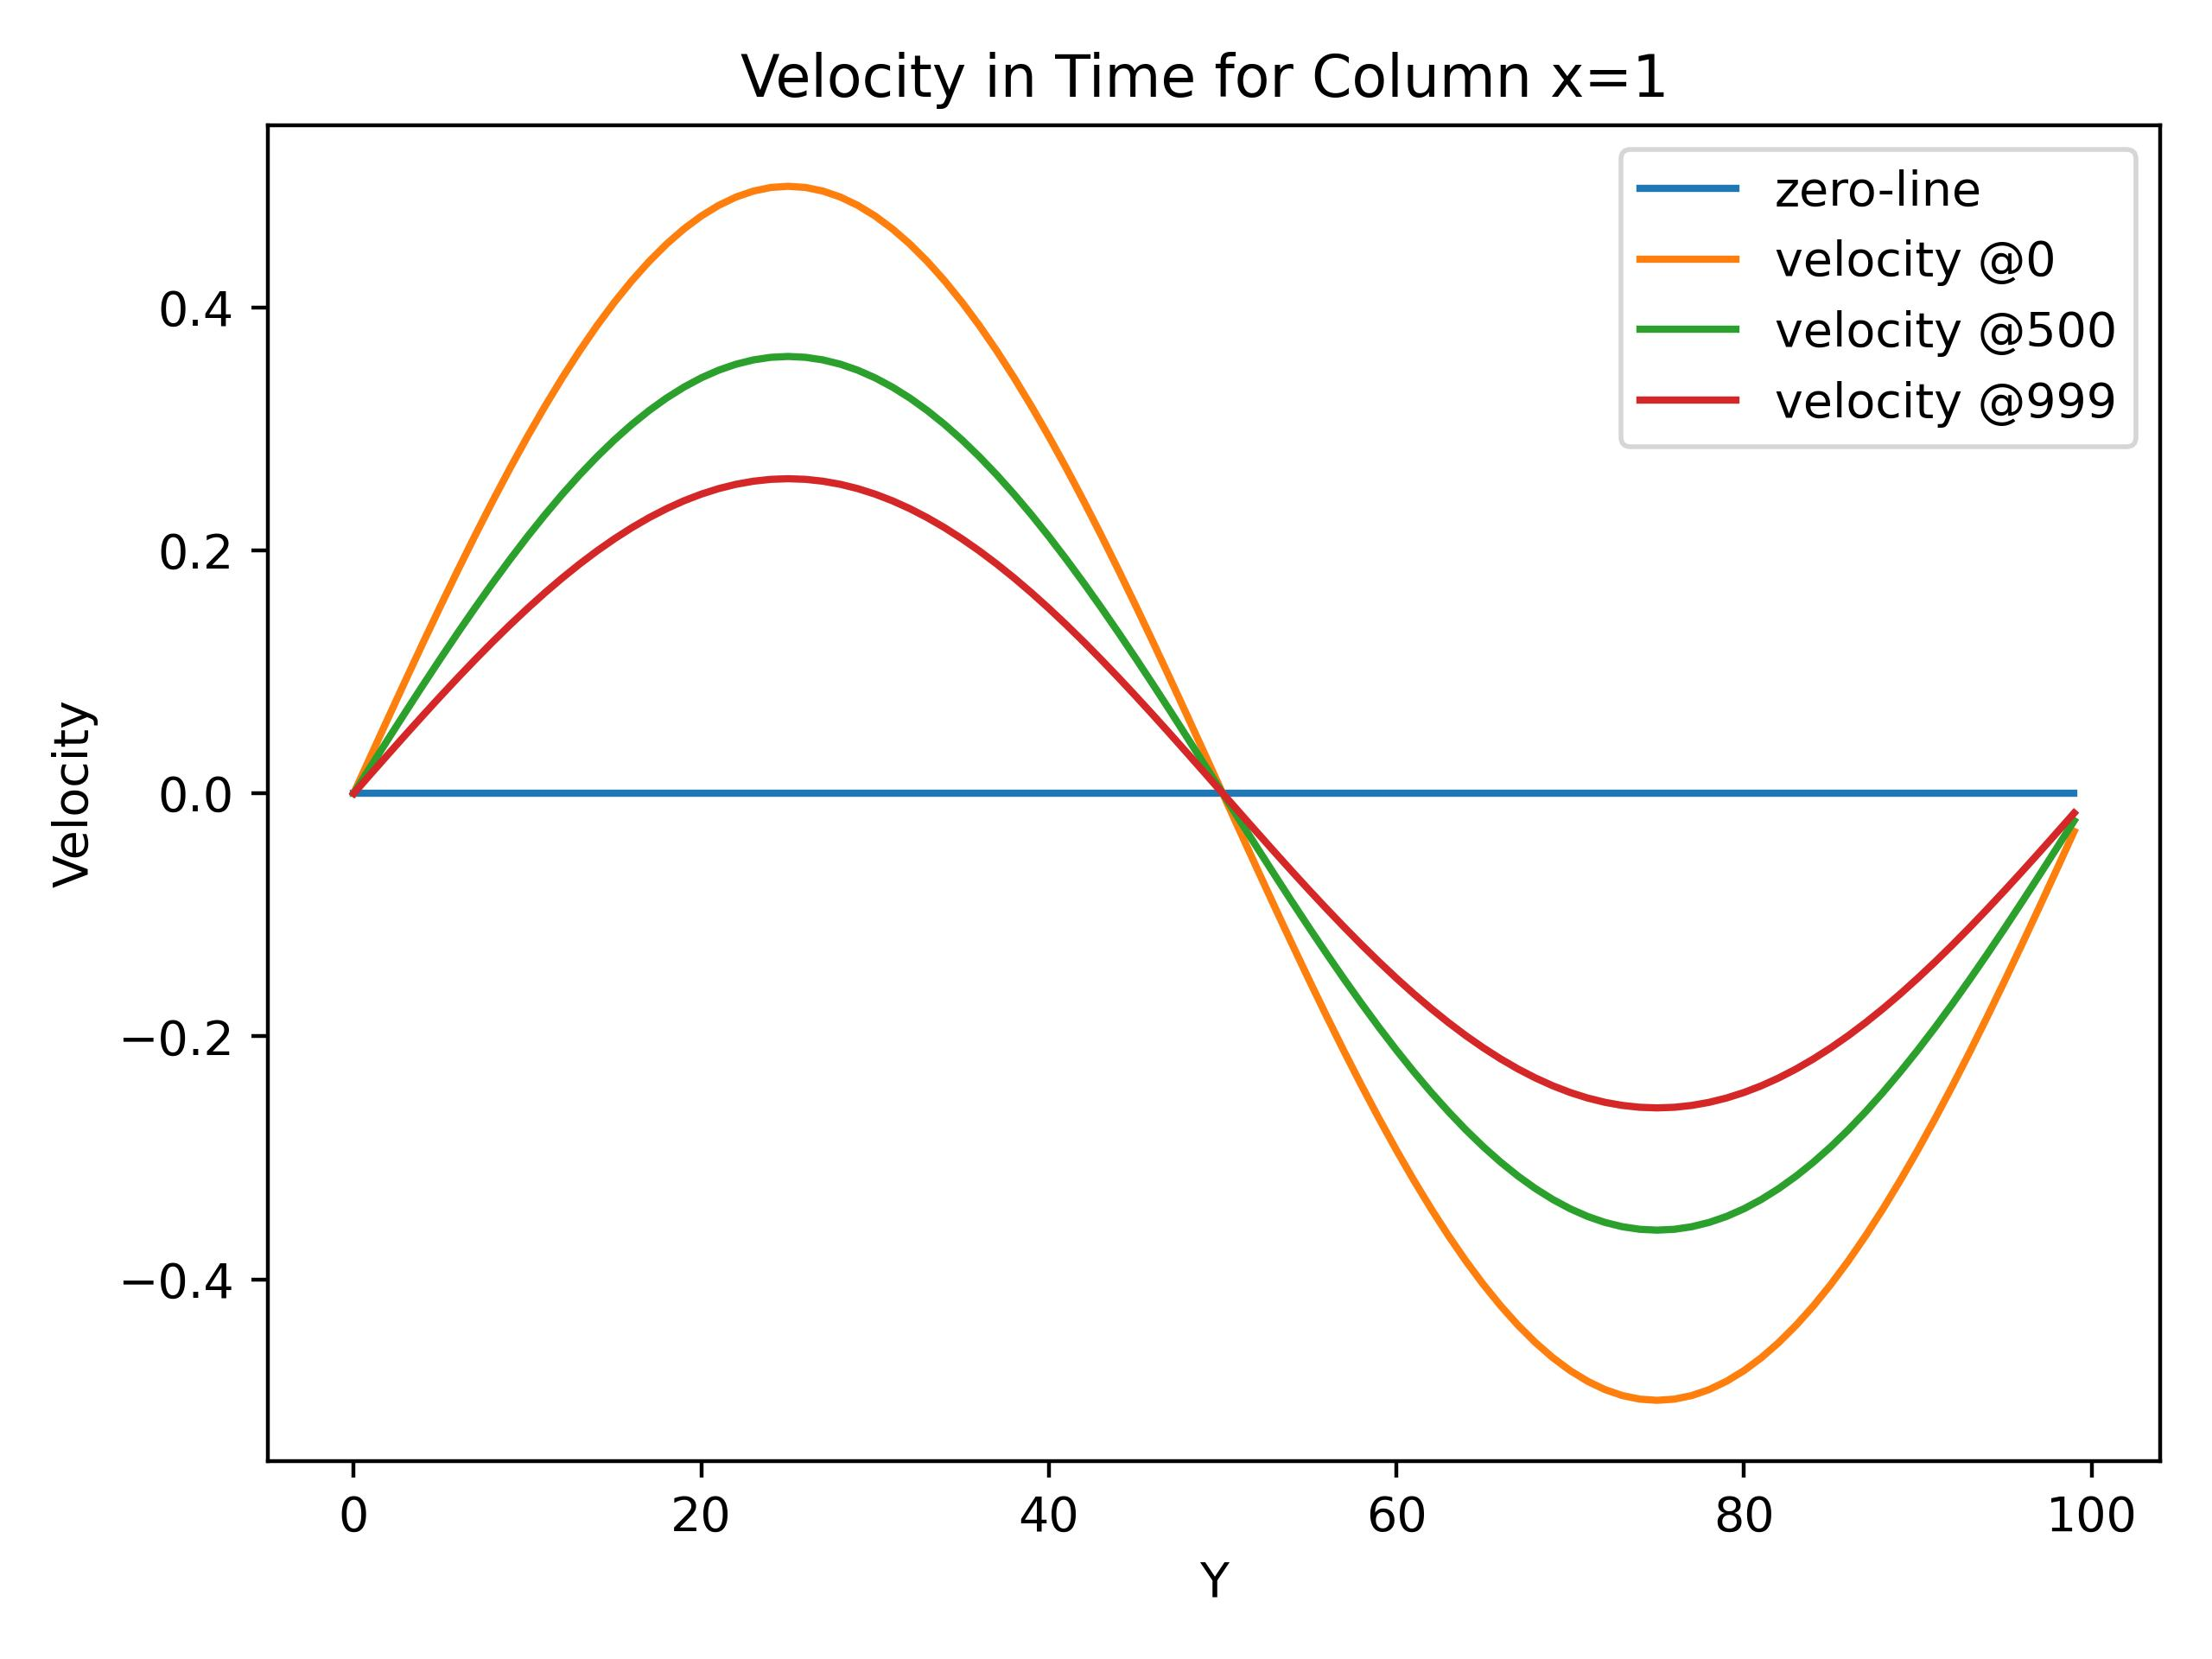
\includegraphics[width=\linewidth]{graphs/ShearWaveDecay/VelocityDistribution/velocity_at_column_x}
            \caption{Decaying velocity at a specific column.}
            \label{fig:swd-vs-at-column_x}
        \end{minipage}% don't remove this comment - uncomments a new line
        \begin{minipage}{0.5\textwidth}
            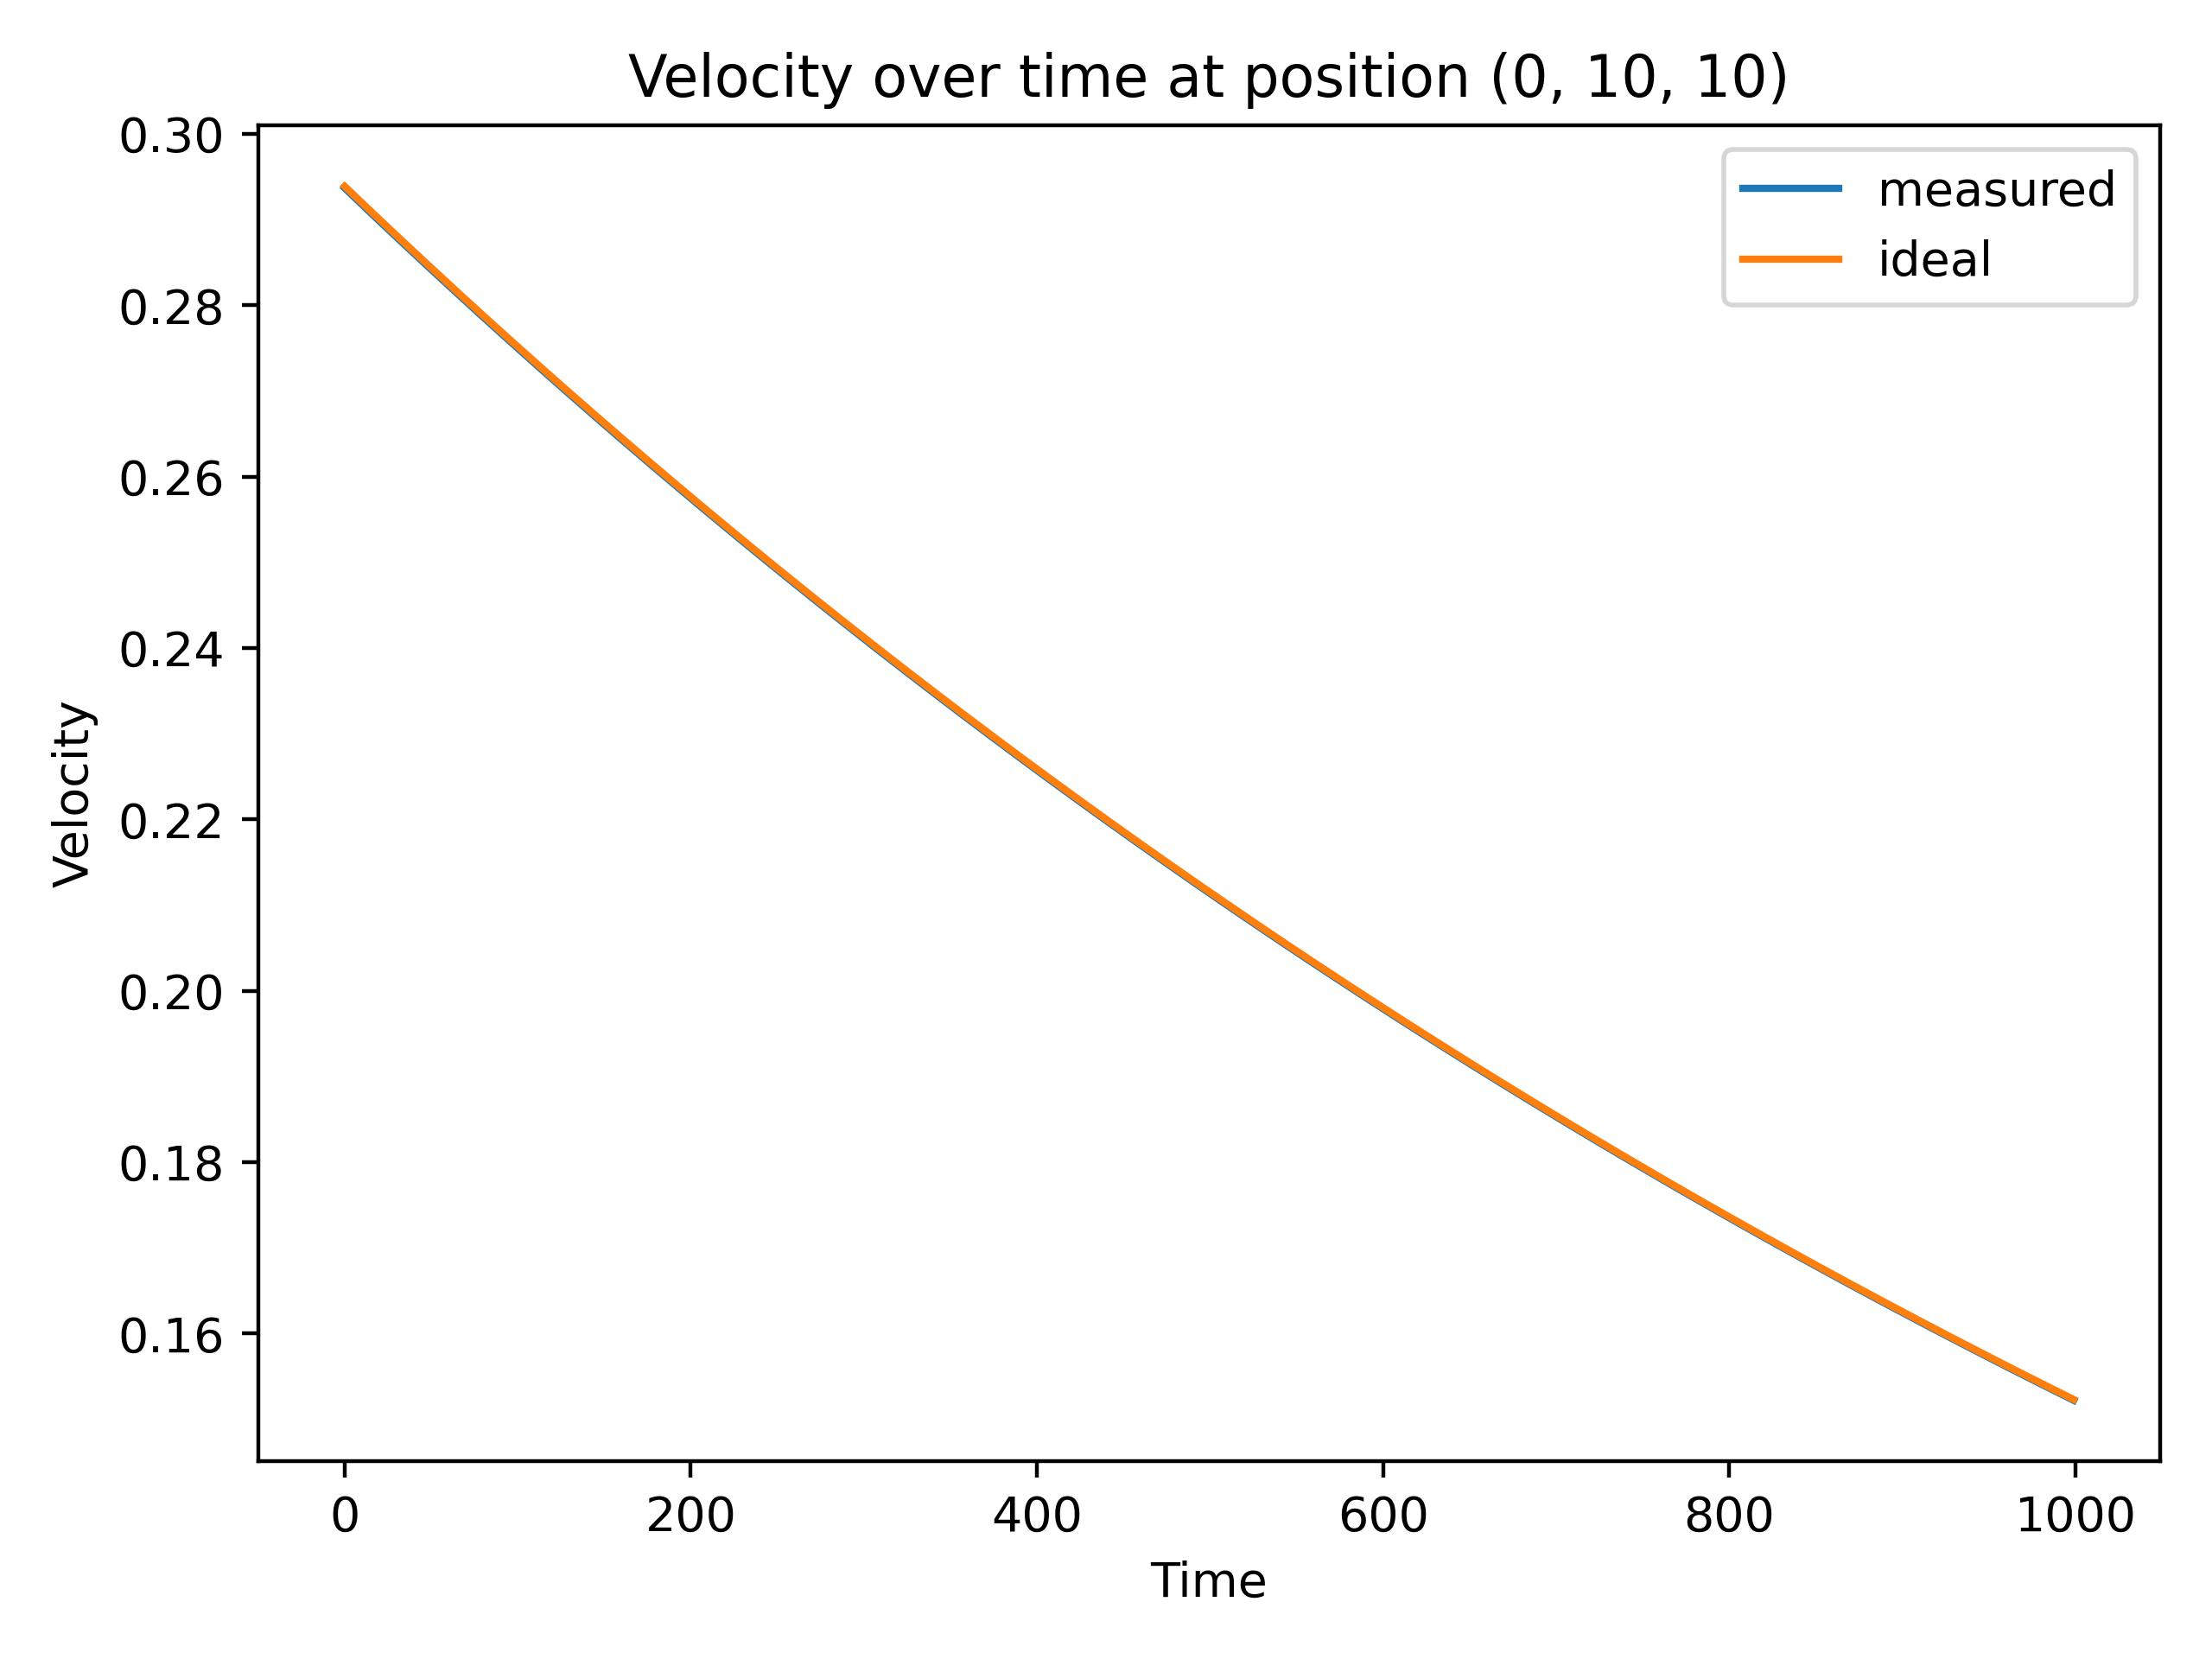
\includegraphics[width=\linewidth]{graphs/ShearWaveDecay/VelocityDistribution/velocity_against_ideal}
            \caption{measured vs ideal decay}
            \label{fig:swd-vs-ideal}
        \end{minipage}
    \end{figure}
\end{center}

\subsection{Correlation of Kinematic Viscosity and Omega}
% TODO in methods: equation to calculate viscosity from experiment
This experiment aims to measure the correlation between the kinematic viscosity and the parameter omega, that is used for the collision.
The kinematic viscosity describes, how \textit{thick} some fluid is, e.g.\ syrup has a higher viscosity than water. % https://en.wikipedia.org/wiki/Viscosity
This experiment measures the viscosity by running the previous experiment \cref{subsec:sinusoidal-velocity} multiple times with different omegas.
It is expected that a lower omega has a higher viscosity. % TODO why?
The results of the experiment are shown in \cref{fig:swd-vo-viscosity-vs-omega}.

\begin{figure}[h!]
    \begin{center}
        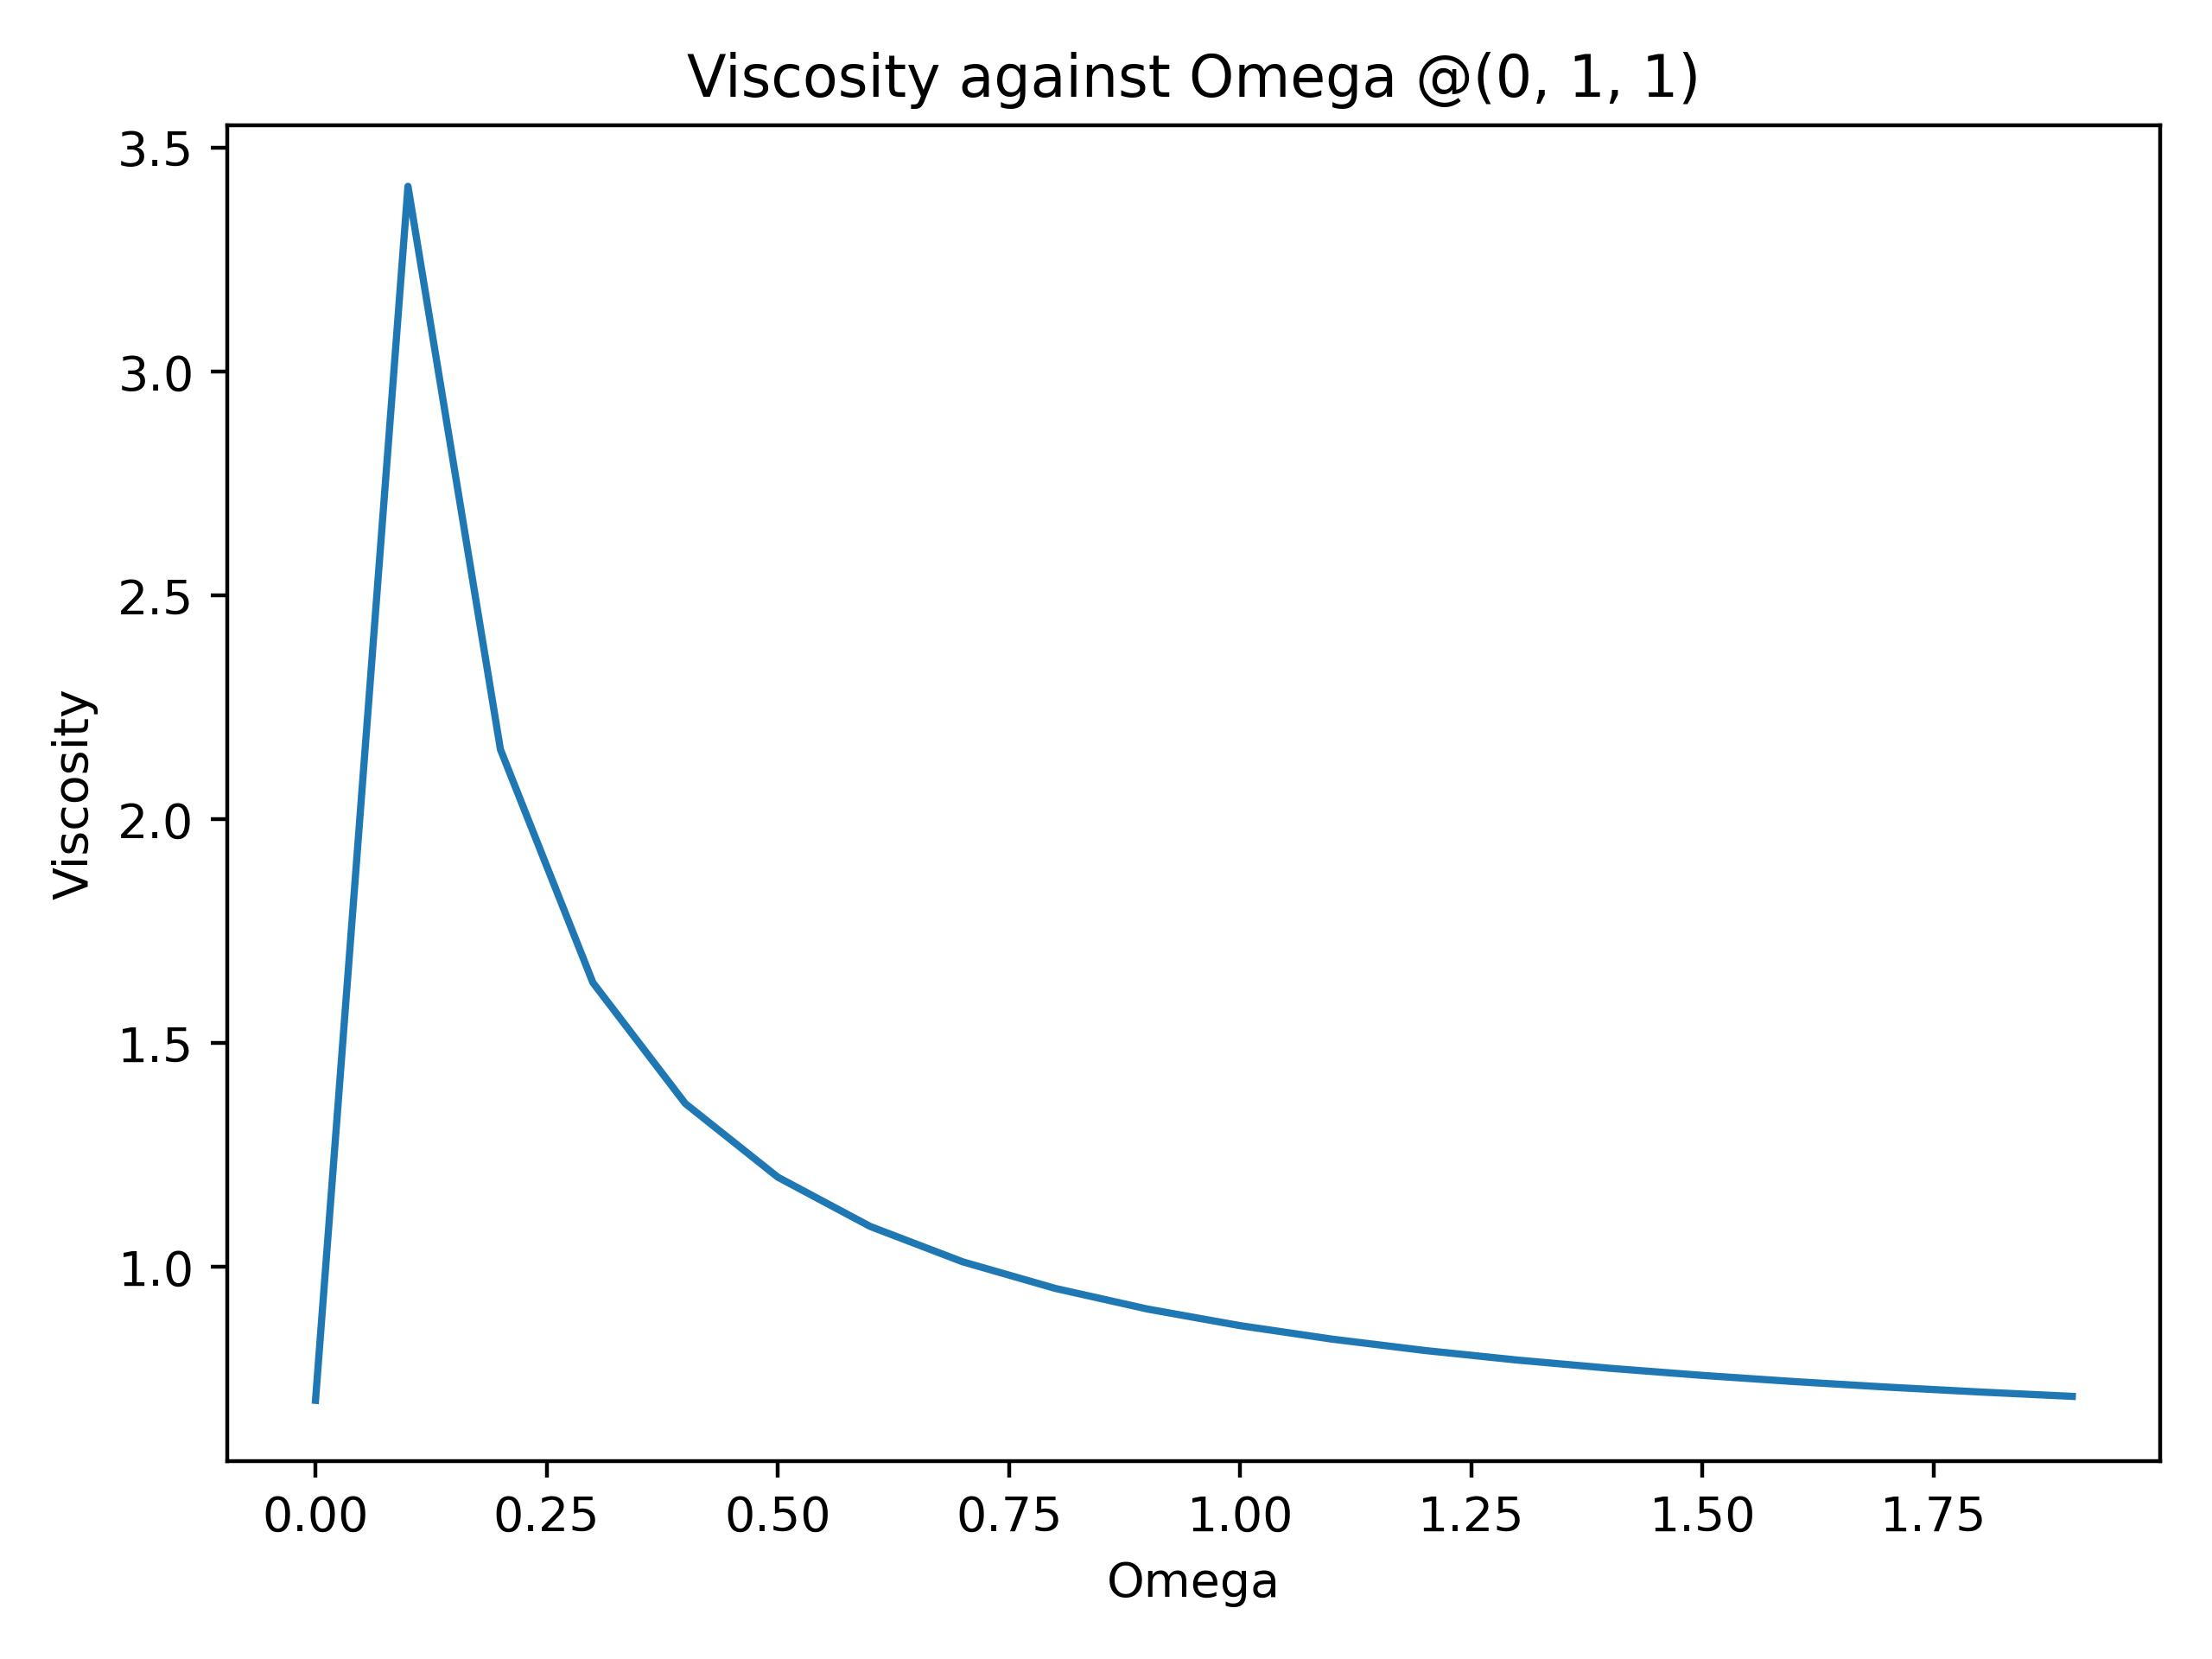
\includegraphics[width=0.5\linewidth]{graphs/ShearWaveDecay/Viscosity/viscosity_against_omega}
        \caption{Correlation between the kinematic viscosity and omega.}
        \label{fig:swd-vo-viscosity-vs-omega}
    \end{center}
\end{figure}

Strangely, for very small omega, the viscosity does not follow the otherwise exponential decay.
This is due to the model of the simulation, that fails to replicate the exact behaviour with too large or small values. % TODO why?
In theory, this may even have an impact on the experiments, but omega was set to 1.0 to not have a negative impact of this phenomenon.
